\documentclass{article}

\usepackage[left=2cm, right=2cm, top=1cm]{geometry}
\usepackage[utf8]{inputenc}
\usepackage{amsmath}
\usepackage{enumitem}
\usepackage{float}


\title{Snowman Fourier Study Sheet Exam 1}
\author{Hannah Gallagher}
\date{October 1st, 2024}

\usepackage{natbib}
\usepackage{graphicx}

\begin{document}

\maketitle

\section{Introduction}

%Convolution 
%Eigenvalues Eigenvectors 
%Discrete fourier transform 
%Continuous transform 
%Vector basis 
%Circulant matrix
%Euler relation



% Hot keys to remember: command / on a mac comments highlighted code in and out.
Nugget the snowman wishes you good luck on your exam!

\begin{figure}[h!]
\centering
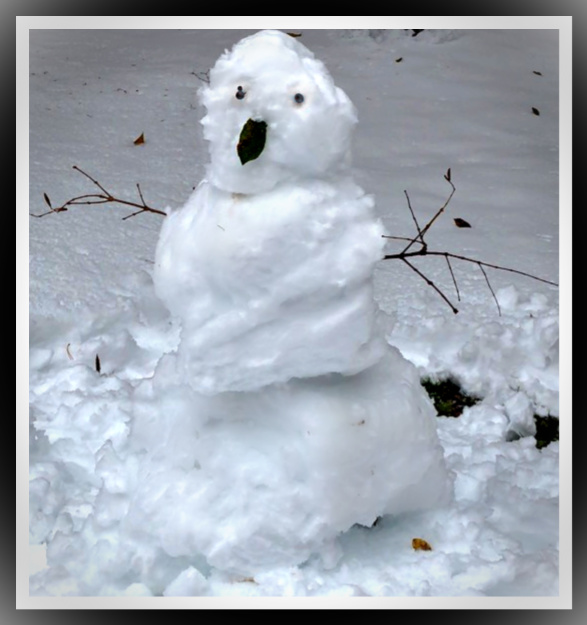
\includegraphics[scale=1]{Nugget.jpg}
\caption{Nugget the Snowman}
\label{fig:Nugget}
\end{figure}

\section{Given Information, Key Terms, and Things to Remember} 
\begin{itemize}
\item Argand diagrams and roots of unity.
\item Inverse problems are the most involved. 
\item The problem of expressing $cos [4 \pi \theta ]$ in only theta. 
\item The quadratic phase graph.
\item Cycles per pixel. 
\item Circulant matrices.
\item Diagonalizing a matrix
\item Dirac Delta and graphs. 
\item STEP function and graphs. 
\item TRI function and graphs. 
\item RECT function and graphs. (even) 
  \begin{itemize}
    \item This is an even function
    \item He loves it being piecewise as well.
  \end{itemize}

\begin{figure}[h!]
\centering
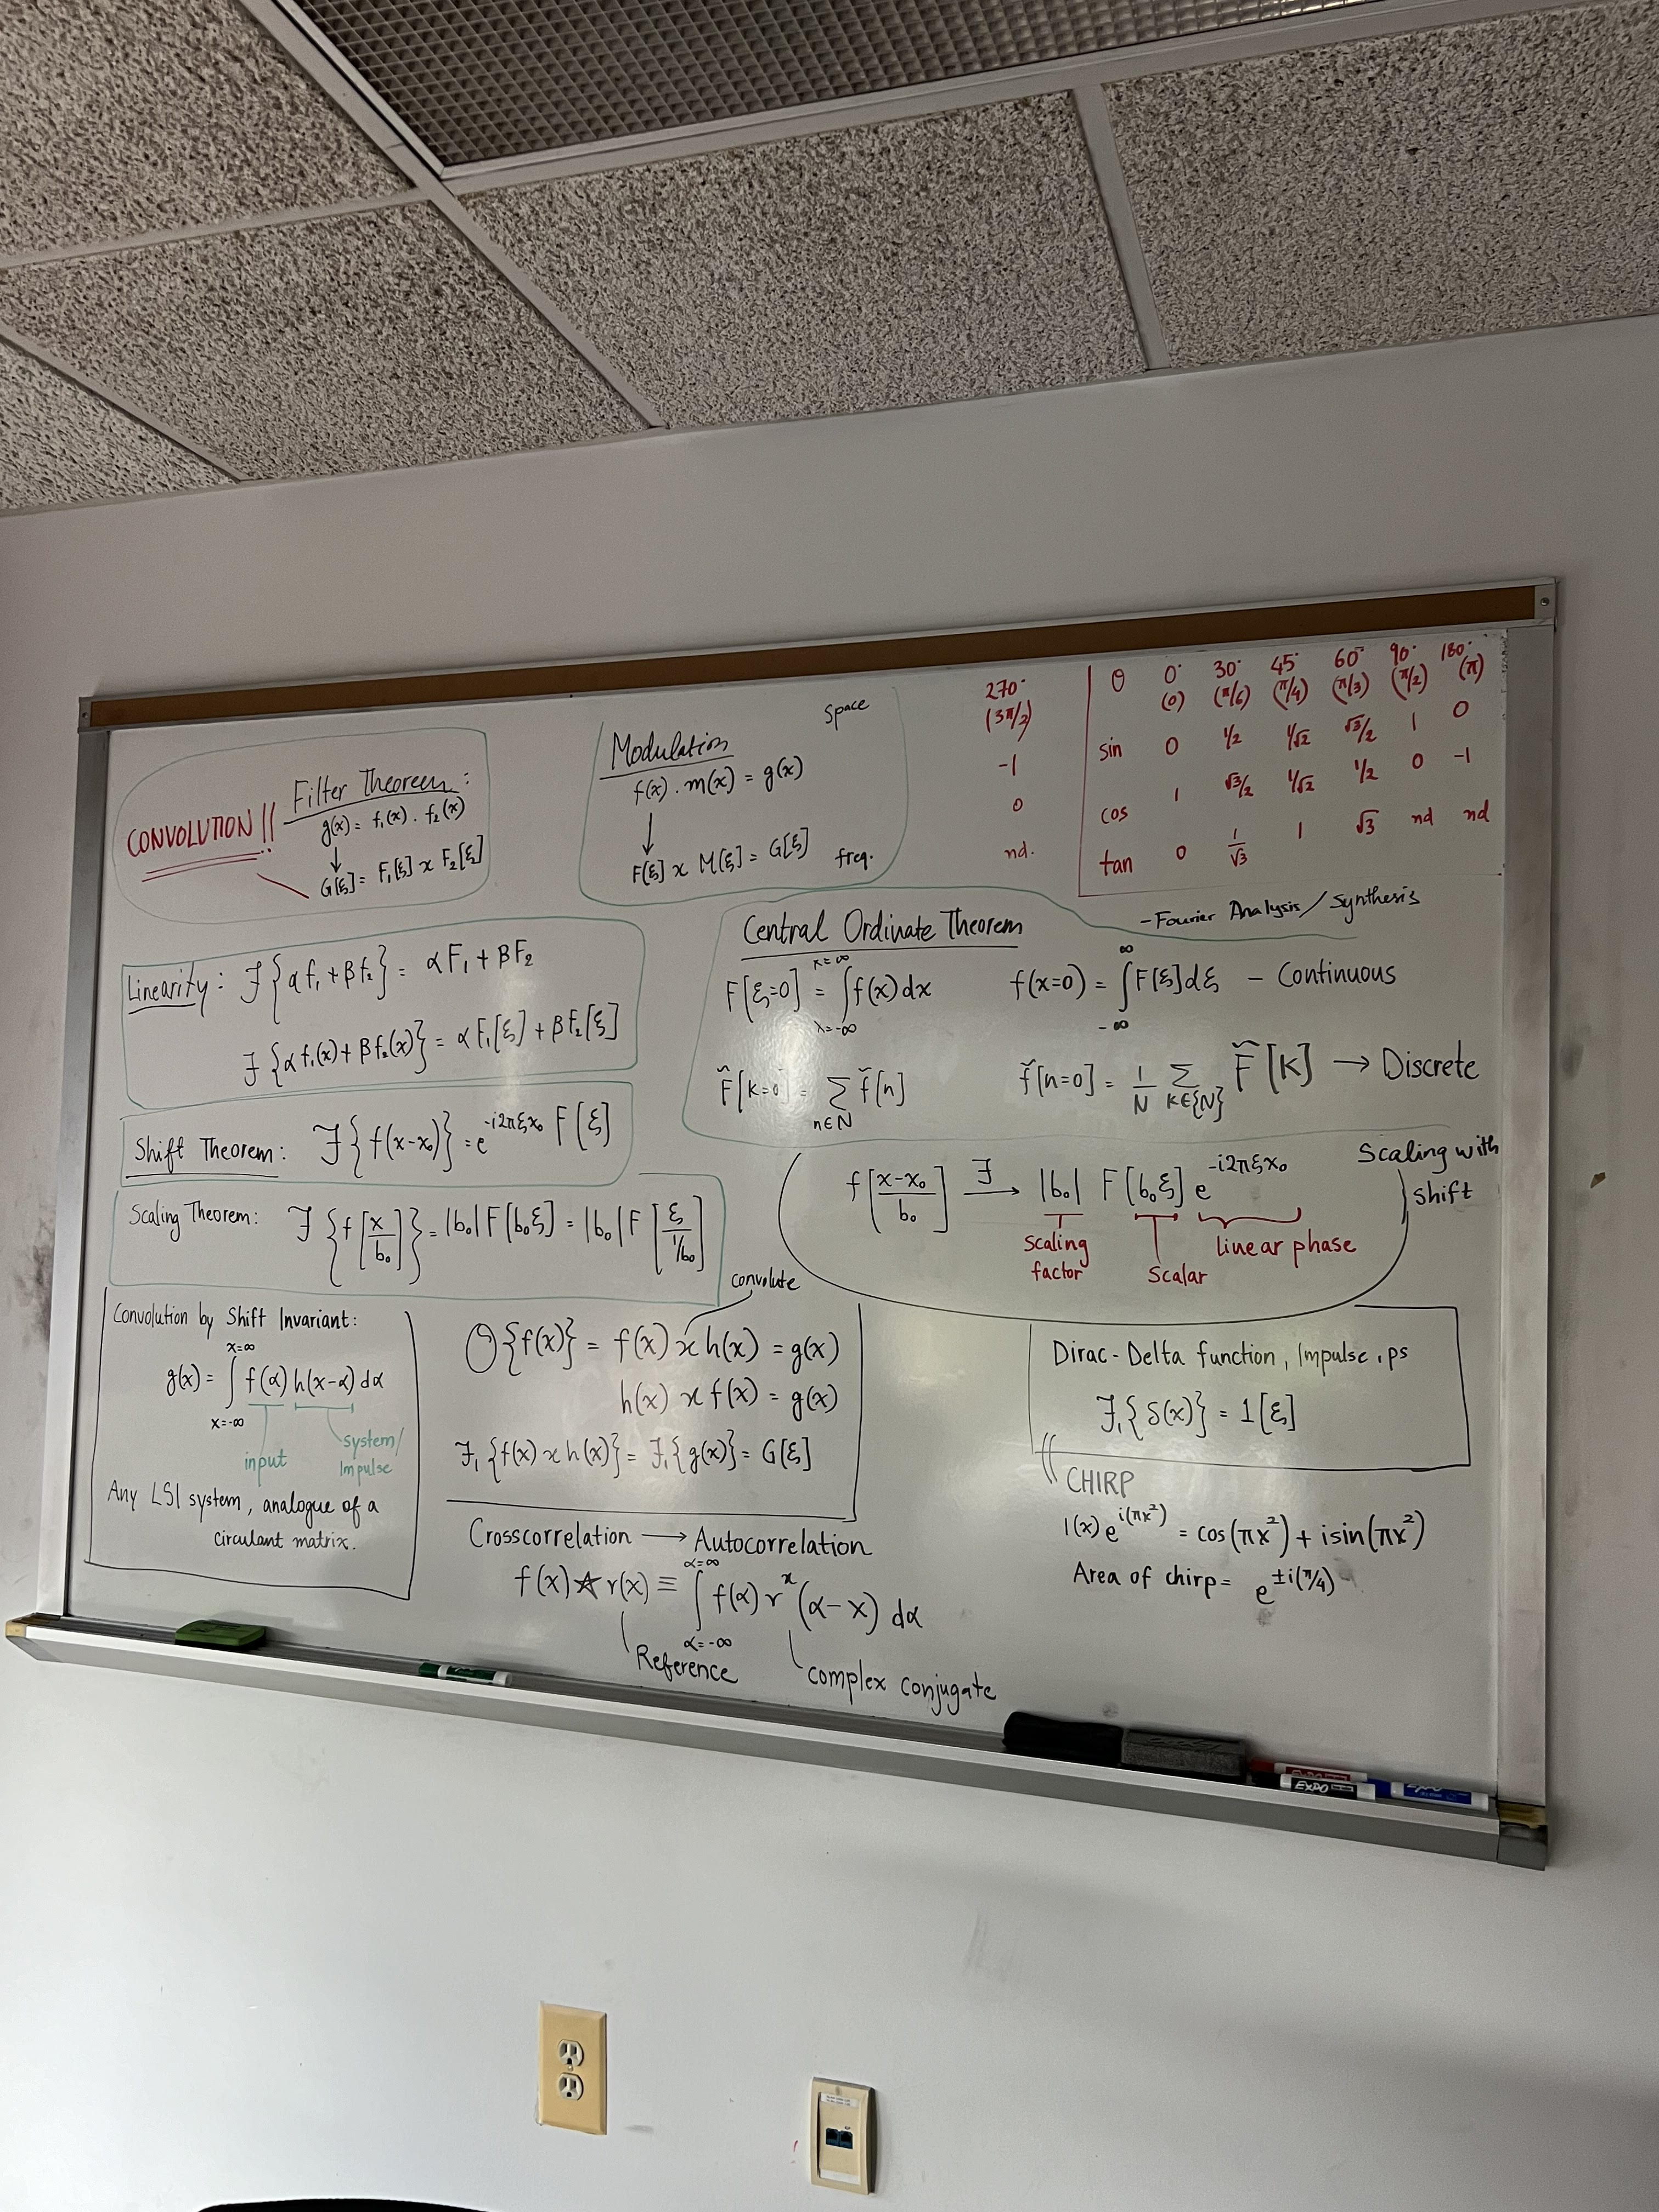
\includegraphics[scale=.20]{Fourier/unnamed.jpg}
\caption{Easton Syllabus}
\label{fig:Snowmanda}
\end{figure}


 
\end{itemize}




\clearpage
\section{Homework's Day By Day}
\subsection{Homework 1}
\subsubsection{Rectangle function}


\subsubsection{Even and Odd Functions}


\subsubsection{Translation of Functions}



\subsubsection{Adding a Series to get the Square Wave}



\subsubsection{Magnitude and Phase Angles}


\subsubsection{Projection}


\subsubsection{Dot Product}




\subsubsection{Lexicographic Ordering of Matrices}



\subsubsection{Whether the Inverse of a Matrix Exists}



\subsection{Homework 2}


\subsubsection{Finding the Input and Output Vector in a Matrix}






\section{Notes Day by Day}

\subsection{August 27th, 2024}
\subsubsection{The Imaging Chain} 

Source of Energy or Object

Propagation 

Collection or Optics 

(Propagate) 

Sensor: This converts energy to the "Signal"

Processing: Compression of JPEG or MPEG

Perception

\subsubsection{Phase angle}

\subsubsection{Quadratic Phase}

\subsubsection{Unit Vectors}


\subsection{September 3rd, 2024}



\subsection{September 10th, 2024}


\subsection{September 17th, 2024}
The dark room one. 
Introduction of the delta function. 
More graphs. 
Something about the Fourier transform of $e^{i 2 \pi -\xi_{0}x}$ = $\delta(\xi_{0}+\xi_{0})$

$e^{i 2 \pi \xi_{0}x} + e^{-i 2 \pi \xi_{0}x} = 2 cos(2 \pi \xi_{0}x)$ $\longrightarrow$ $\delta(\xi-\xi_{0}) + \delta(\xi+ \xi_{0})$

$1(x)e^{i (\pi x^2)}= \cos(\pi x^2) + i \sin(\pi x^2)$

\subsection{September 24th, 2024}
Right before the exam. 



Things to remember: 
The Fourier Transform of $RECT[x]$ is $SINC[\xi]$

The Fourier Transform of $SINC[x]$ is $RECT[-\xi]$ which is equivalent to $RECT[\xi]$

The Scaling Theorem tells us that $f[\frac{x}{b_0}] = |b_o| F[\frac{\xi}{1/b_{0}}]=|b_0|F[b_{0}\xi]$ where $b_0 \neq 0$

$f[\frac{x}{-1}]= f[-x] \rightarrow F[-\xi]$
$-f[x] \rightarrow - F[\xi]$

If simply multiplied by a constant $A_0$: 
Then $A_0 f[x] \rightarrow A_0 F[\xi]$ is just a fact of LINEARITY. 

Shift Theorem: 
$f[x- x_{0}] \rightarrow F[\xi] e^{-i 2 \pi \xi x_{0}}$


Phase Angle: 

$\Phi{F[\xi]} = \arctan (\frac{Im{F[\xi]}}{Re{F[\xi]}})$

Delta Function: 

$\delta[x] \rightarrow 1[\xi] + i0[\xi]$
Impulse 

$\delta[x-x_{0}] \rightarrow 1[\xi] e^{-i2 \pi \xi x_{0}} = \cos[2 \pi \xi x_{0}+ i[-\sin[2 \pi \xi x_{0}]]]$

$\Phi{F[\xi]}= -2 \pi \xi x_{0}$ is proportional to $\xi$


$e^{- 2 \pi x \xi_{0}} \rightarrow \delta((-\xi)-\xi_{0}) = \delta(\xi +\xi_{0})$


$\int_{-\infty}^{+ \infty} f[\alpha] \delta[x- \alpha] d \alpha = f[x]$

Constraints 

1) Linearity $\sigma{A_{0}f[x]}= A_0 g[x]$
2) Shift Invariance $\sigma {f[x- x_{0}]} = g[x-x_{0}]$

LSI 

$\sigma {f[x]}= g[x]= \sigma {\int_{- \infty}^{+ \infty}f[\alpha]\delta[x- \alpha]d \alpha}$




\subsubsection{WHY DOES THE PHASE ANGLE CHANGE?} 

Shifting property 

By Shift invariance 

$g(x) = \int ^{\infty}_-{\infty}f(\alpha) h(x- \alpha) d \alpha$ Convolution. 
Which any LSI system, is the analogue of the circulant matrix. 

Then you do the change of variable to evaluate that convolution. 


\subsection{October 8th, 2024}

After the exam. 

$G[\xi] = F[\xi] \dot H[\xi] = delta[\xi - \xi_{0}H[\xi]]$



\subsection{November 19th, 2024}
Types of filters. 
Mentions a possible exam question. With some sort of chirp on the function.  



\subsubsection{LSI}


\subsubsection{Filter Theorem}

\subsubsection{Gaussian was not on the exam: Please study this} 
1 hour in

\subsubsection{Noise Stochastic Signals}

\subsubsection{Linear and Shift Invariant then the output is also zero cannot create new data}
\subsubsection{Fourier Synthesis}

\begin{equation}
    \huge\Sigma^{N-1}_{k=0} F[k]= \frac{1}{\sqrt{N}}e^{+i 2 \pi n \frac{k}{N}}= f[n]
\end{equation}




\clearpage
\section{Mostly Unedited Syllabus}
\begin{figure}[h!]
\centering
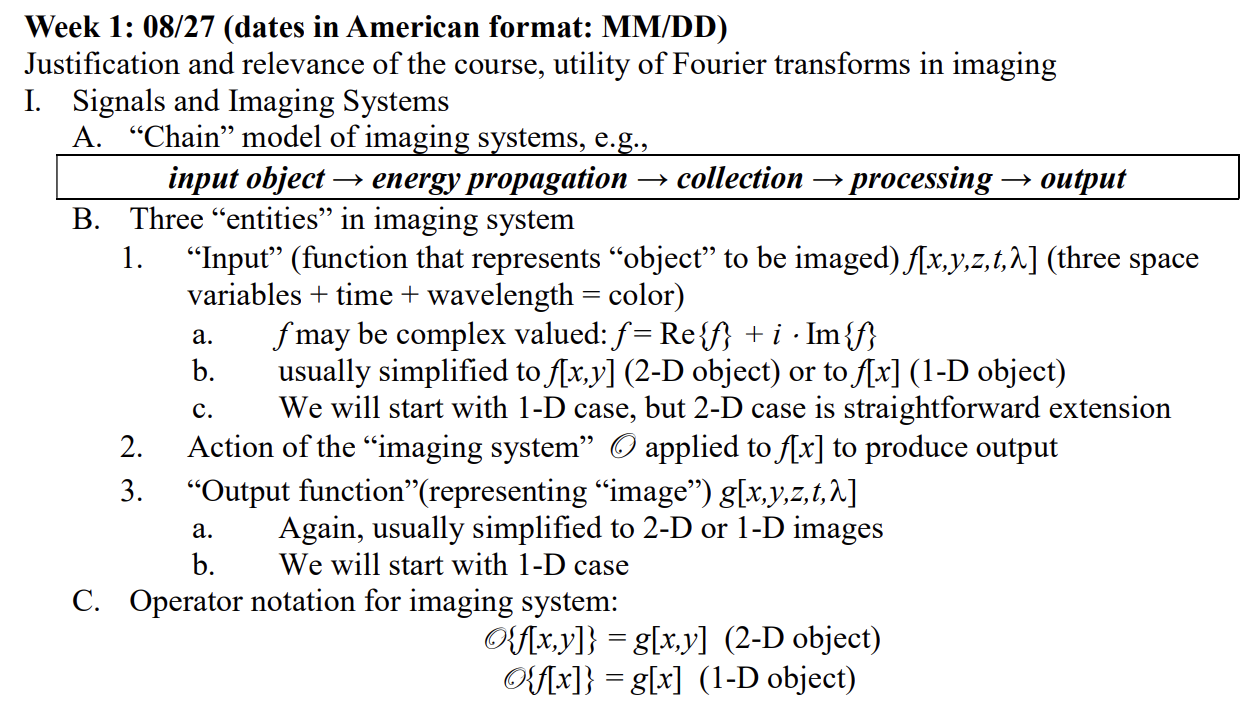
\includegraphics[scale=.60]{Fourier/Week 1/Week1.1.png}
\caption{Easton Syllabus}
\label{fig:Snowman1}
\end{figure}


\begin{figure}[h!]
\centering
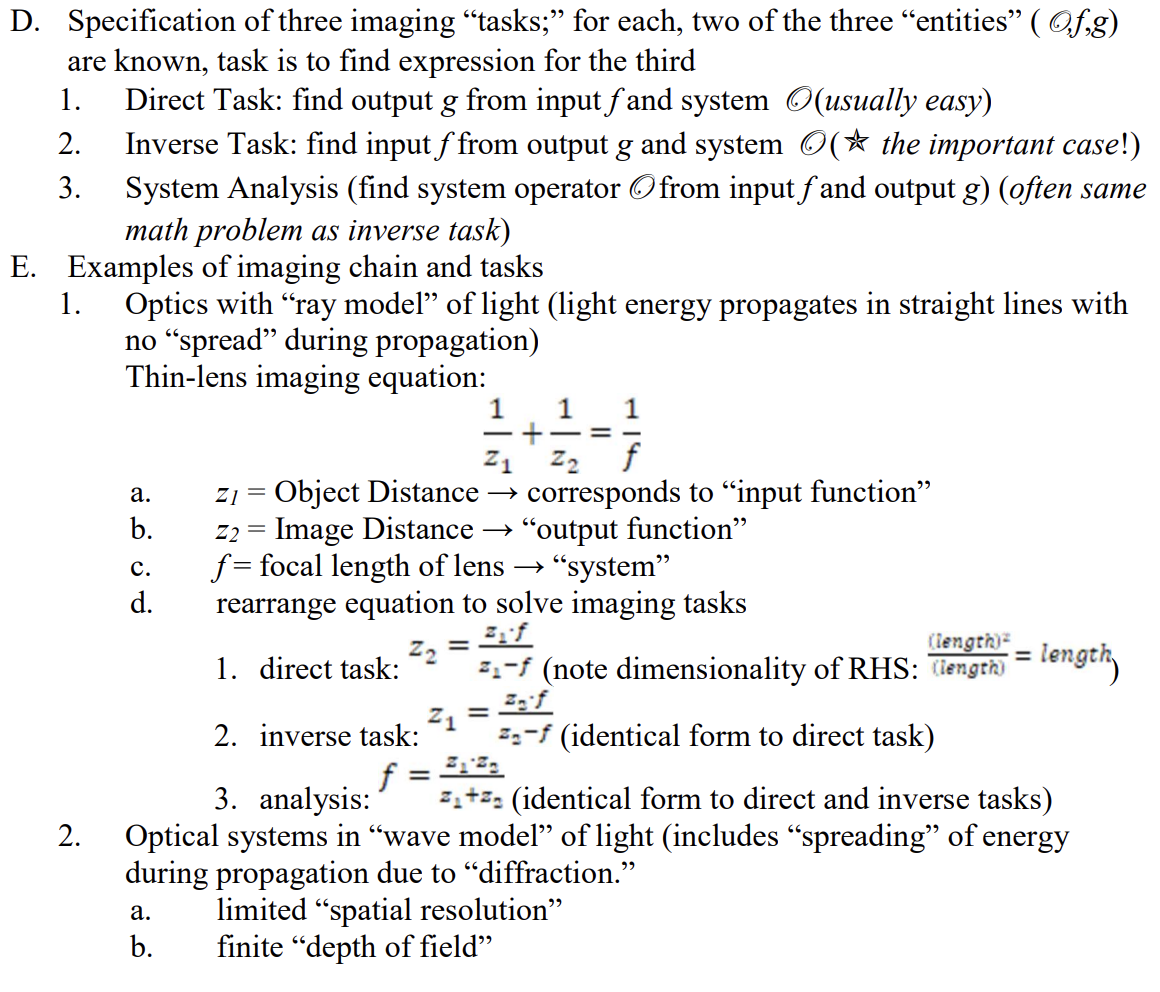
\includegraphics[scale=.60]{Fourier/Week 1/Week1.2.png}
\caption{Easton Syllabus: Most of this is geometric optics as a review. We focus on the inverse task for most of the more difficult problems. The limited spatial resolution needs to be looked into. I am not sure if he is referencing the error with the hubble space telescope.}
\label{fig:Snowma2n}
\end{figure}

\begin{figure}[h!]
\centering
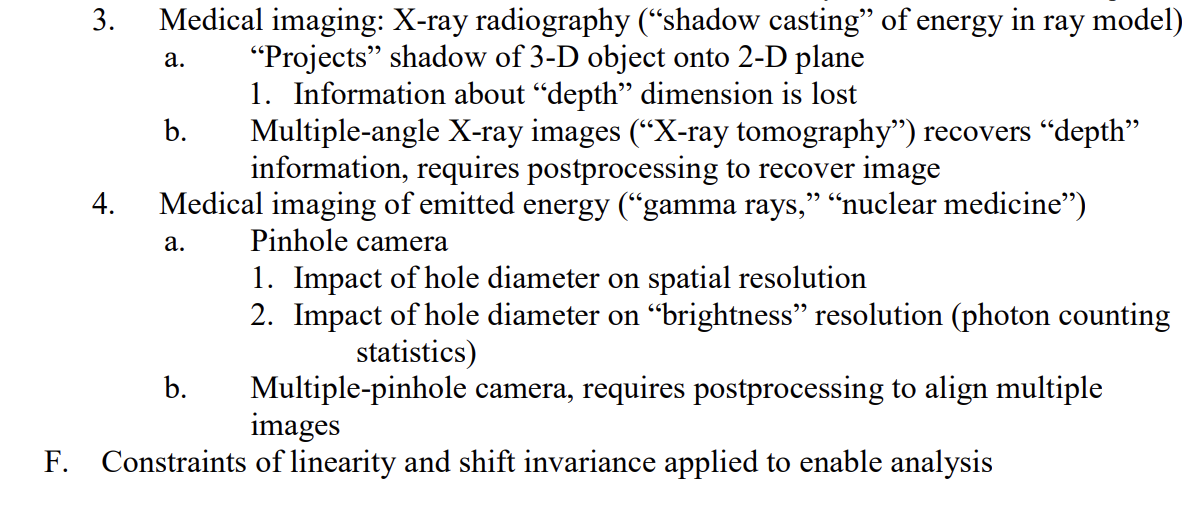
\includegraphics[scale=.65]{Fourier/Week 1/Week1.3.png}
\caption{Easton Syllabus: FOCUS ON MRI MATRIX EXAMPLE}
\label{fig:Snowman2}
\end{figure}

\begin{figure}[h!]
\centering
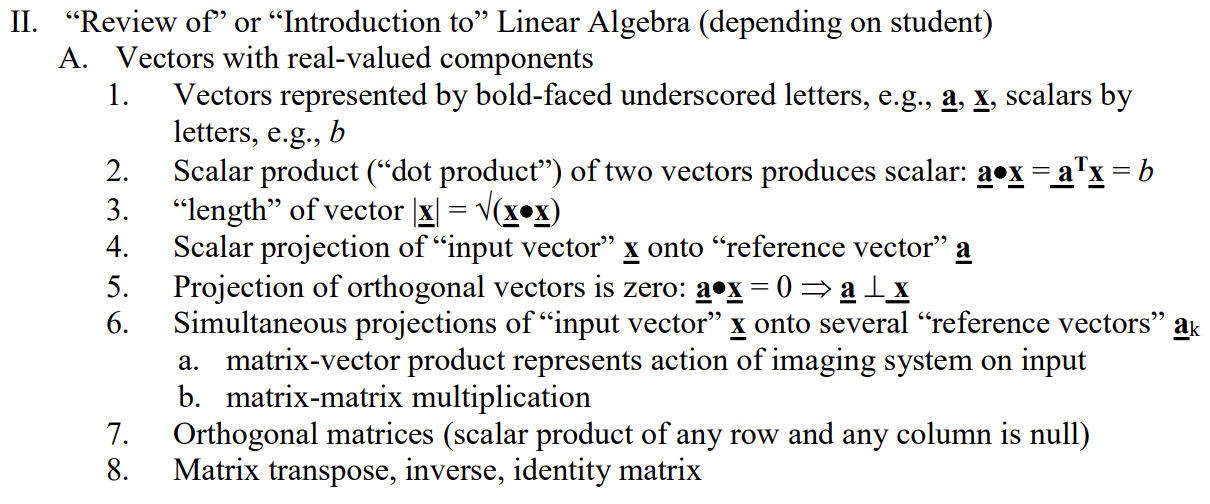
\includegraphics[scale=.65]{Fourier/Week 1/Week1.4.png}
\caption{Easton Syllabus: The basics of Linear Algebra and Matrices}
\label{fig:Snowman3}
\end{figure}

\begin{figure}[h!]
\centering
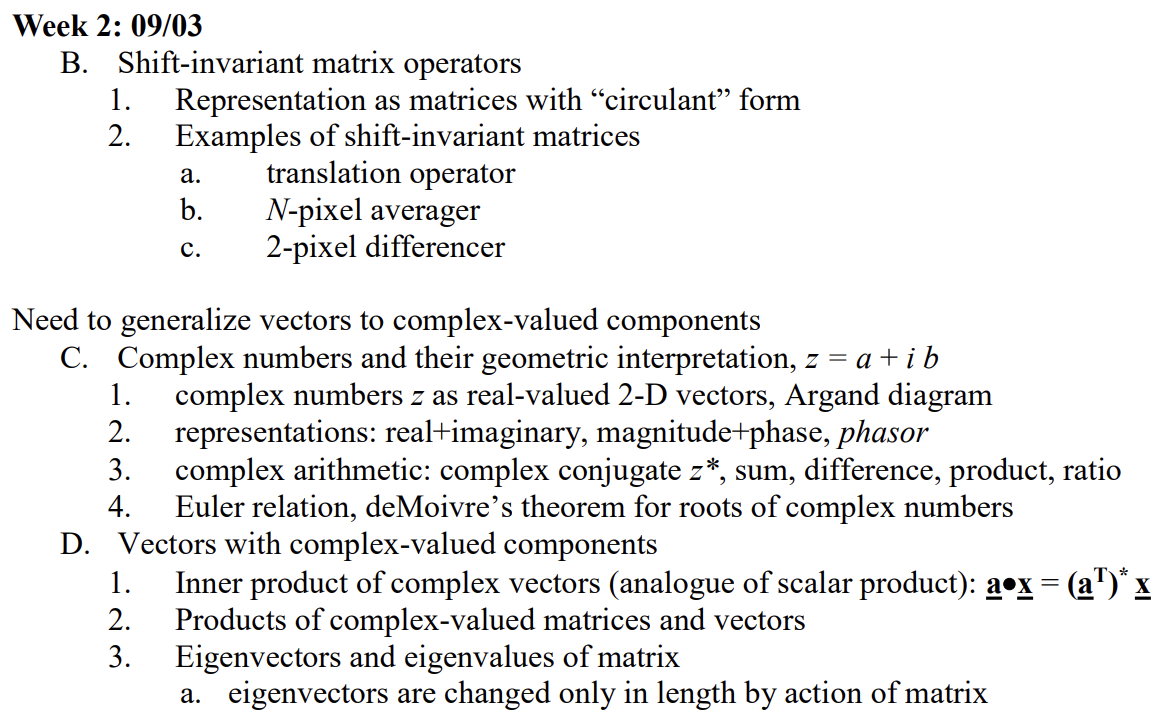
\includegraphics[scale=.65]{Fourier/Week 2/Week2.1.png}
\caption{Easton Syllabus: Argand Diagram and Euler Relation}
\label{fig:Snowman4}
\end{figure}

\begin{figure}[h!]
\centering
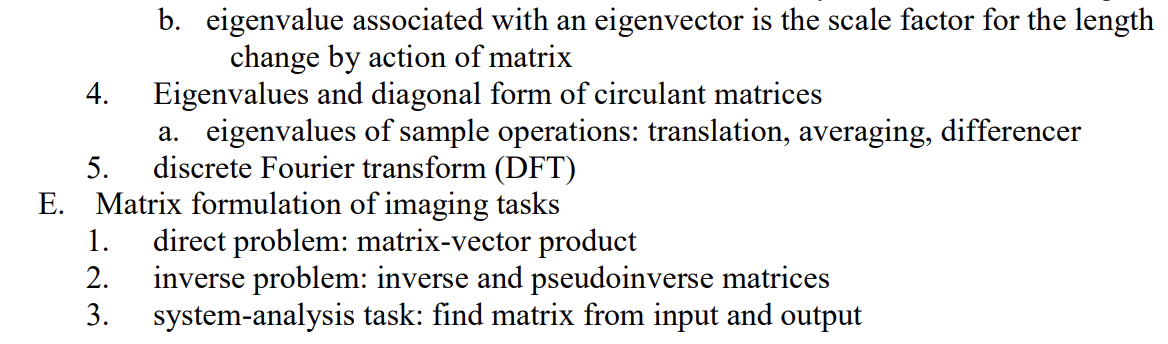
\includegraphics[scale=.65]{Fourier/Week 2/Week2.2.png}
\caption{Easton Syllabus: Pseudoinverse matrices, DFT equation}
\label{fig:Snowman5}
\end{figure}

\begin{figure}[h!]
\centering
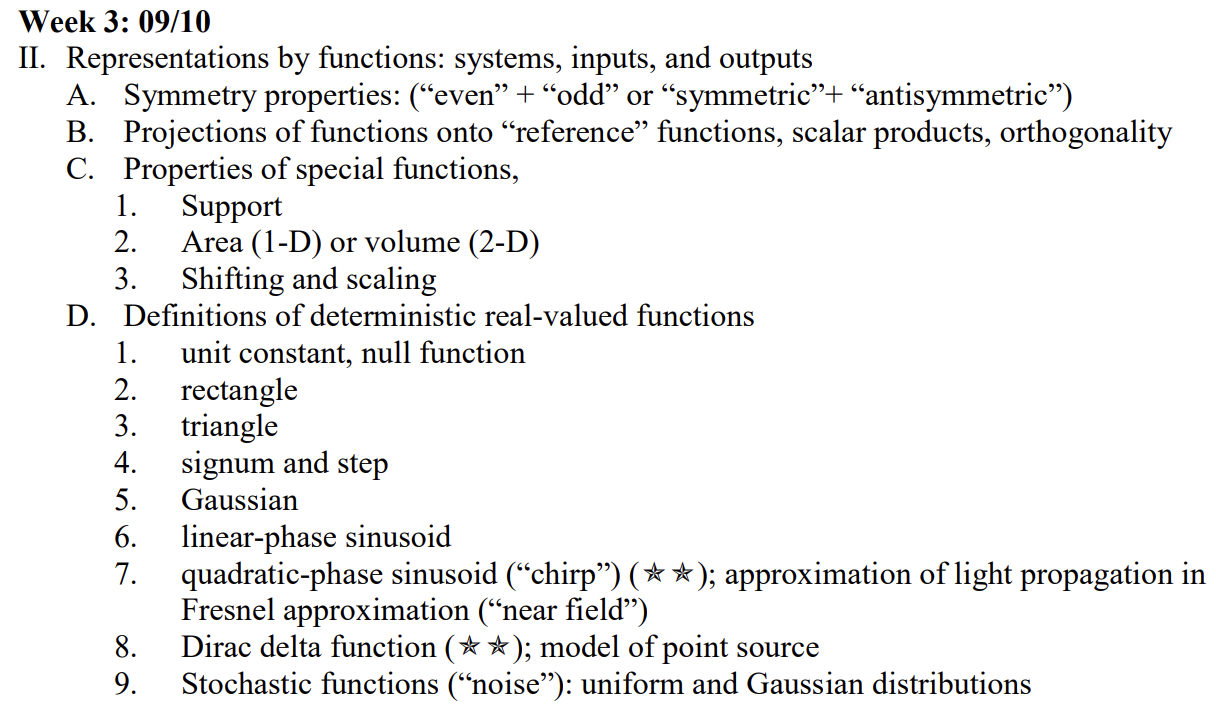
\includegraphics[scale=.65]{Fourier/Week 3/Week3.1.png}
\caption{Easton Syllabus}
\label{fig:Snowman6}
\end{figure}

\begin{figure}[h!]
\centering
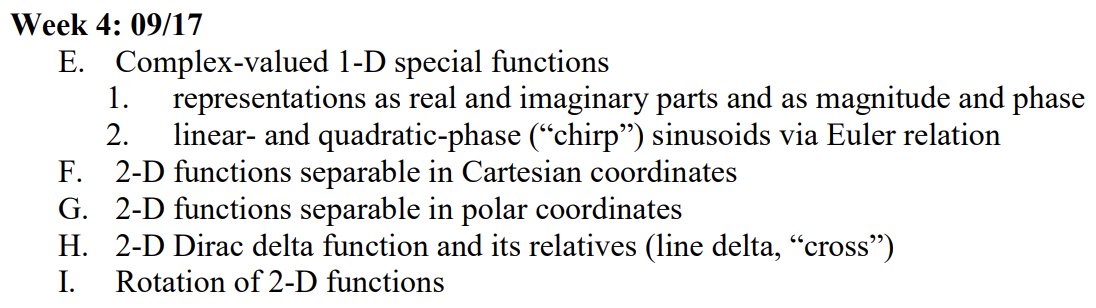
\includegraphics[scale=.65]{Fourier/Week 4/Week4.1.png}
\caption{Easton Syllabus}
\label{fig:Snowm6an}
\end{figure}

\begin{figure}[h!]
\centering
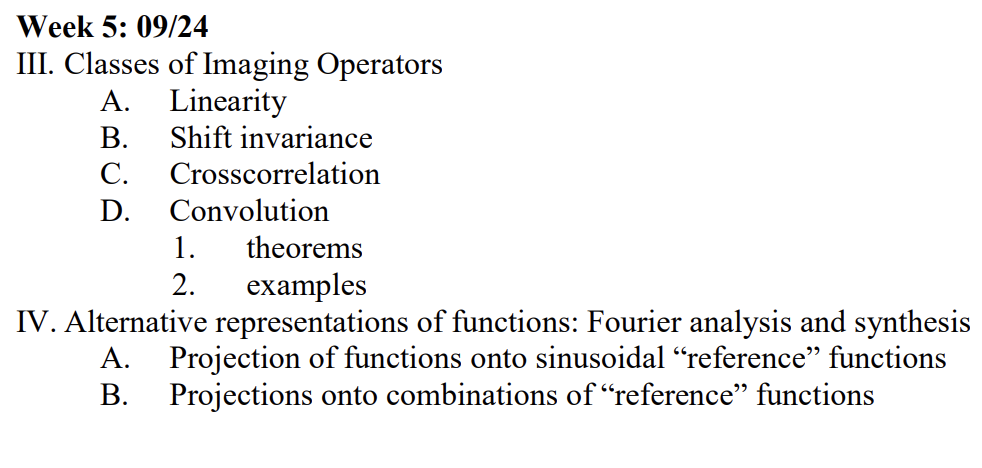
\includegraphics[scale=.65]{Fourier/Week 5/Week5.1.png}
\caption{Easton Syllabus}
\label{fig:Syllabu7s}
\end{figure}


\begin{figure}[h!]
\centering
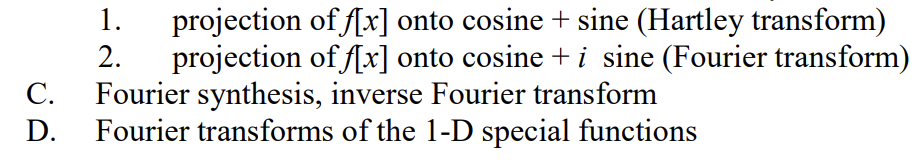
\includegraphics[scale=.65]{Fourier/Week 5/Week5.2.png}
\caption{Easton Syllabus}
\label{fig:Syllab4us}
\end{figure}


\begin{figure}[h!]
\centering
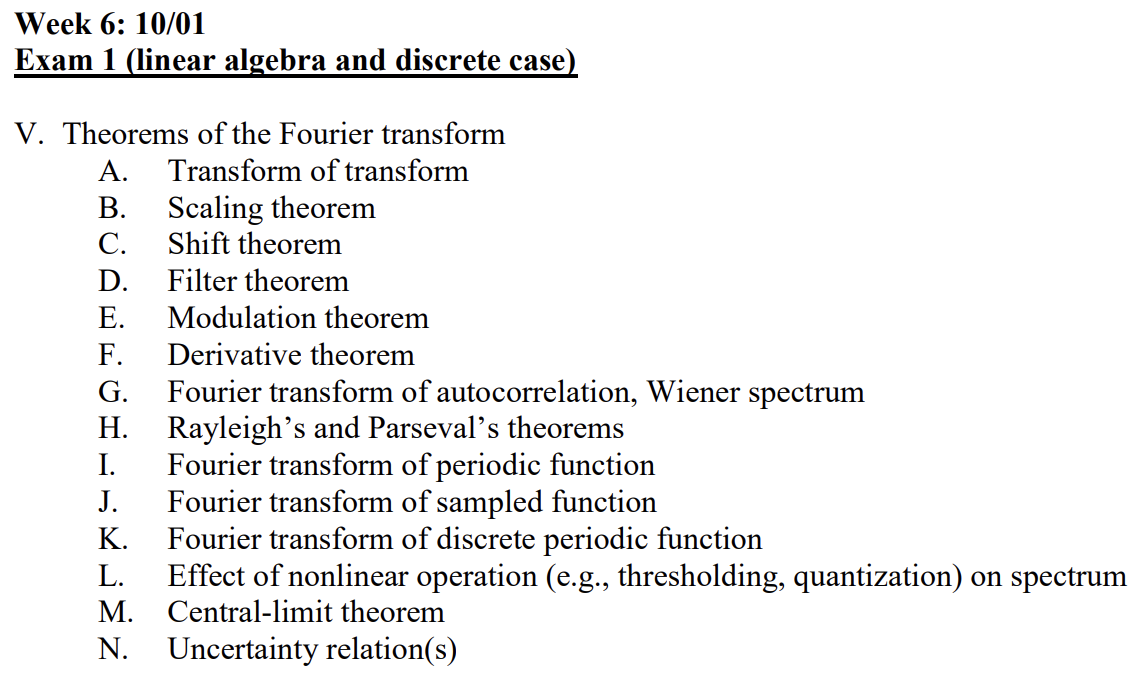
\includegraphics[scale=.65]{Fourier/Week 6/Week6.1.png}
\caption{Easton Syllabus: Wiener Spectrum was emphasized in class.}
\label{fig:Sylla3bus}
\end{figure}


% \newpage
% \section{Medical Imaging Matrix}
% \begin{enumerate}
% \item At what time should Hannah let Meghan work on the middle sphere?
% \item What is the final volume of the snowman?
% \item What is the rate of change of the center sphere's volume at t=3? At t=8? At t=12? 
% \end{enumerate}
 




%\section{Piecewise}

%With everything found so far, it can be explained more compactly in the following piecewise functions.  

%\[ b(t) = \begin{cases} 
%       0 ft & t>1\\
%      .5ft &  t = 1 \\
%      .5ft + .25(t-1) & 1 < t < 7 \\
%      2 ft  & t \geq 7
%   \end{cases}
%\]

% \[ f(t) = \begin{cases} 
%        0 ft & t>1\\
%       .5ft &  t = 1 \\
%       .5ft + .125(t-1) & 1 < t < 5 \\
%       1 ft  & t \geq 5
%    \end{cases}
% \]

% \[ c(t)= \begin{cases} 
%       0 ft & t>1 \\
%       .5ft & 1 \leq t\leq 5 \\
%       .5ft + .125(t-5) & 5 \leq t < 7 \\
%       .75ft + .25(t-7) & 7 \leq t < 11 \\
%       1.75 ft & t \geq 11
%    \end{cases}
% \]





% \section{Formatting}
 

% \[
%     c(t)= .5 +.125(t-5)
% \]   
% \[
%     c= .5 +.125 * (7-5)
% \]   
% \[
%     c= .75 ft 
% \]

% Now, Meghan has a starting radius of .75 ft for the center sphere. 

% \[
%     c= .75ft + .25 * (t-7) 
% \]
% \[
%     c= .75ft + .25 * (11-7)
% \]   
% \[
%     c= 1.75 ft
% \]


% \[
%     V= \frac{4}{3} \pi (b^3 + c^3 + f^3)    
% \]


% \[
%     V= \frac{4}{3} \pi (2^3 + 1.75^3 + 1^3)    
% \]

% \[
%     V= \frac{4}{3} \pi (8 + 5.359375 + 1)    
% \]

% \[
%     V= \frac{4}{3} \pi (8 + 5.359375 + 1)    
% \]

% \[
%     V= 19.1458333 \pi \; ft^3  
% \]



% \section{Question 3}        


% From before, 
% \[
%     V= \frac{4}{3} \pi (r^3)  
% \]

% Let C (t)= Volume of the center sphere at time t. 

% At t= 8 min. 


% \[
%     C = \frac{4}{3} \pi ((.75+.25(t-7))^3)  
% \]

% \[
%     \frac{dC}{dt}= \frac{4}{3} \pi ((.75+ \frac{8-7}{4})^2)\frac{dt}{dt} * (\frac{3}{4}) 
% \]
% \[
%     \frac{dC}{dt}= \pi ((.75+ \frac{t}{4})^2)
% \]

% \[
%     \frac{dC}{dt}= 4\pi (r(t))^2 * r'(t)
% \]

% \[
%     \frac{dC}{dt}= 4\pi (1)^2 * \frac{1}{4}
% \]

% \[
%     \frac{dC}{dt}= \pi \; \; \frac{ft^3}{min}
% \]
\clearpage
\section{Edited Syllabus}
\begin{figure}[h!]
\centering
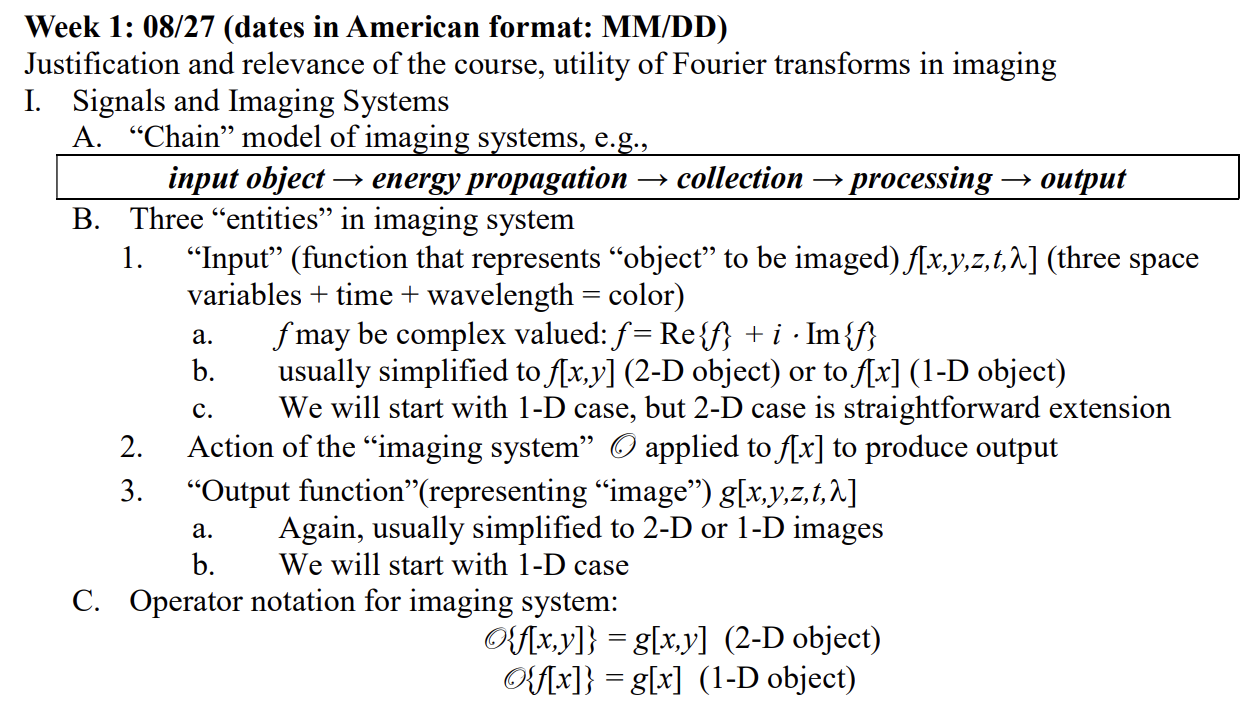
\includegraphics[scale=.60]{Fourier/Week 1/Week1.1.png}
\caption{Easton Syllabus}
\label{fig:Snowman}
\end{figure}


\begin{figure}[h!]
\centering
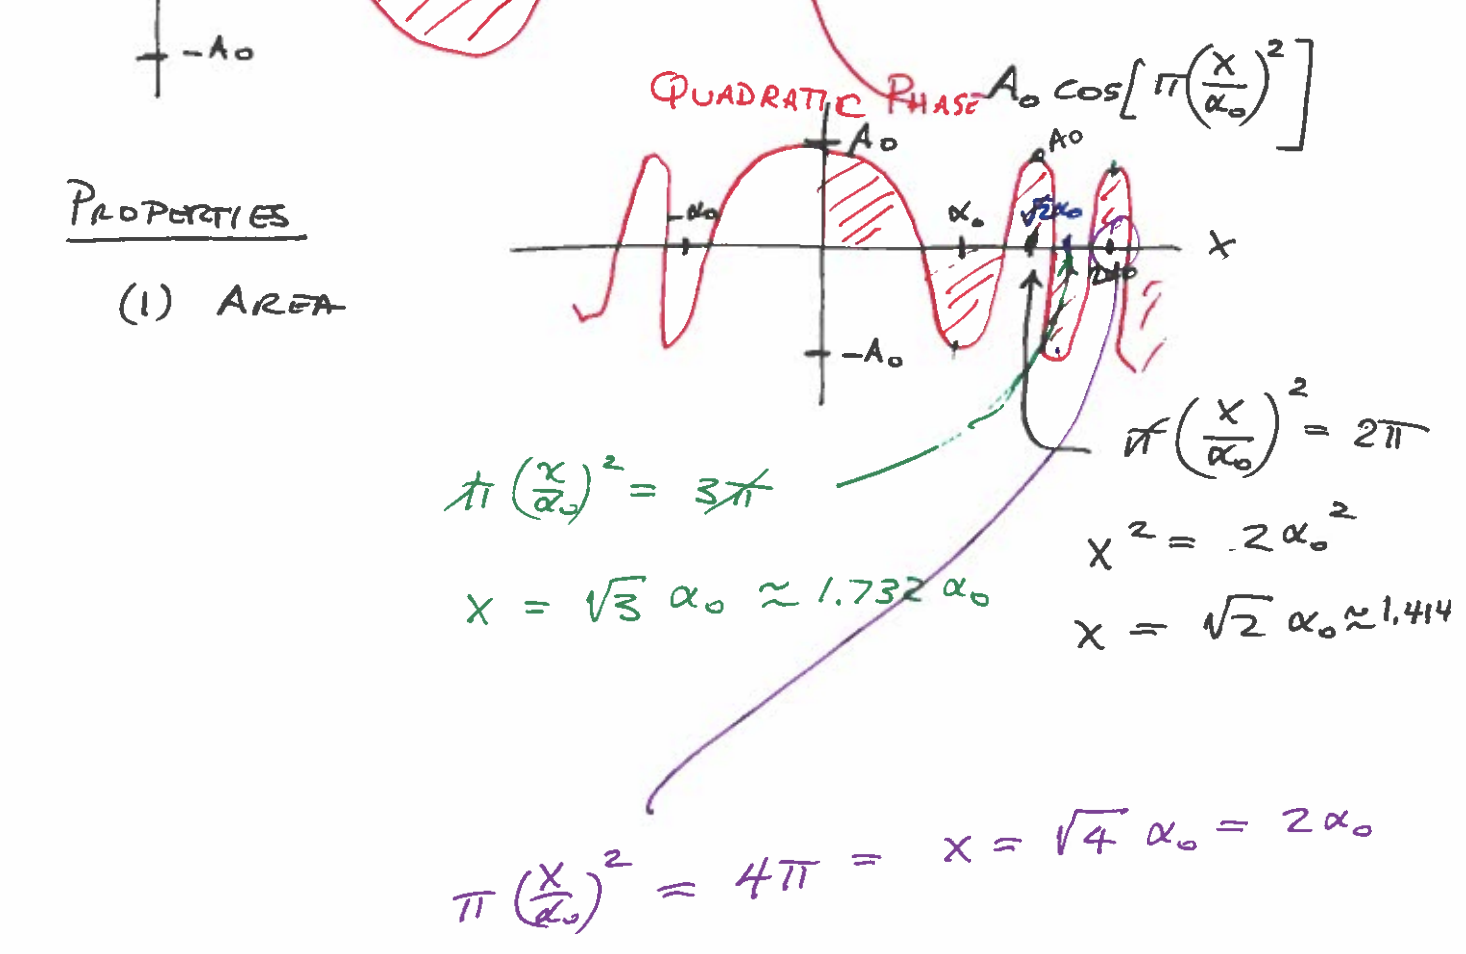
\includegraphics[scale=.65]{Fourier/Week 1/Notes/QuadPhase.png}
\caption{Easton's favorite function: Important in Optics}
\label{fig:QuadPhase}
\end{figure}

\begin{figure}[h!]
\centering
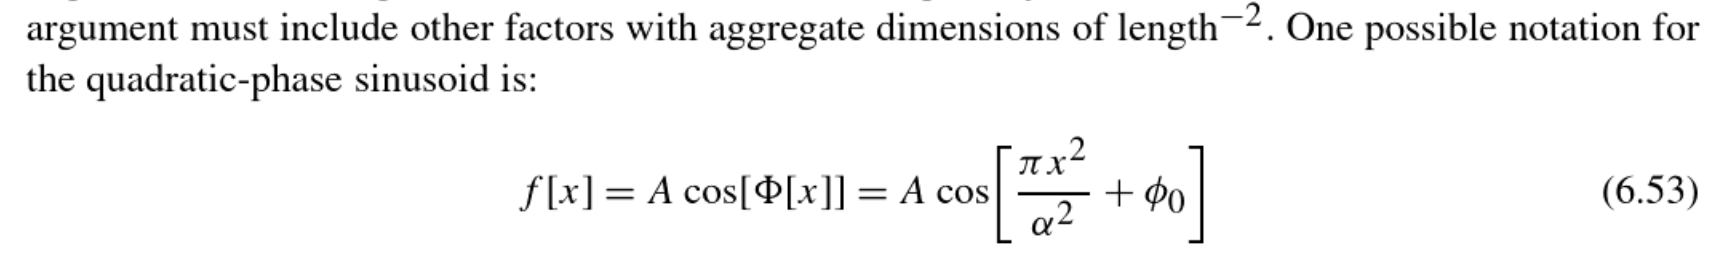
\includegraphics[scale=.65]{Fourier/Week 1/Notes/QuadPhaseEQ.png}
\caption{Easton's favorite function: Important in Optics}
\label{fig:QuadPhas1e}
\end{figure}

\begin{figure}[h!]
\centering
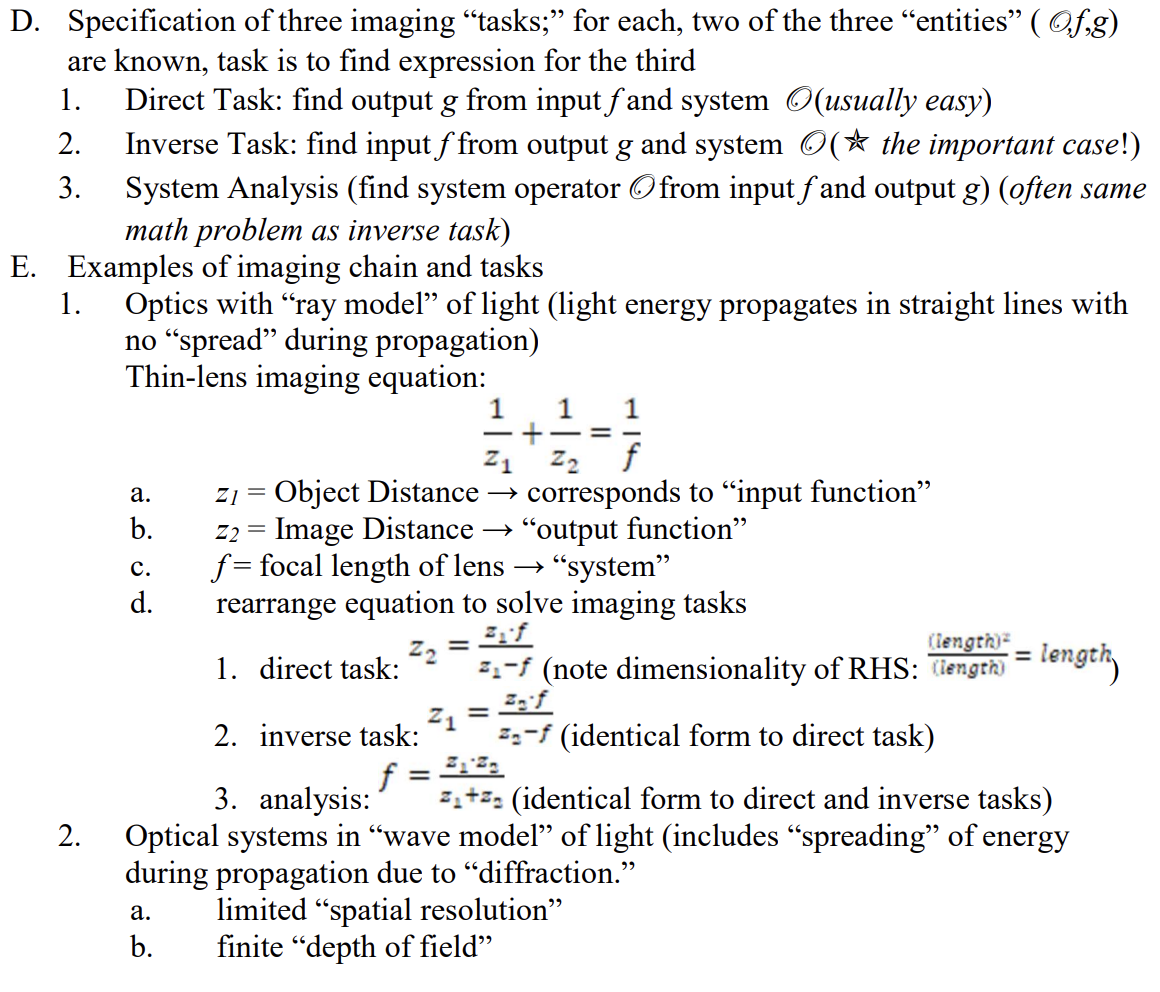
\includegraphics[scale=.60]{Fourier/Week 1/Week1.2.png}
\caption{Easton Syllabus: Most of this is geometric optics as a review. We focus on the inverse task for most of the more difficult problems. The limited spatial resolution needs to be looked into. I am not sure if he is referencing the error with the hubble space telescope.}
\label{fig:Snowman}
\end{figure}

\begin{figure}[h!]
\centering
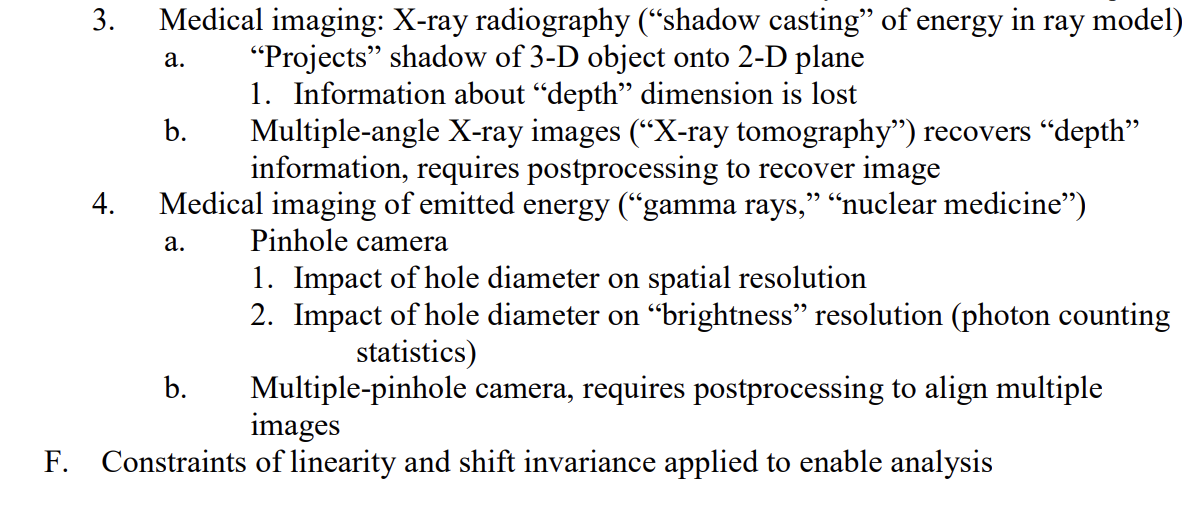
\includegraphics[scale=.65]{Fourier/Week 1/Week1.3.png}
\caption{Easton Syllabus: FOCUS ON MRI MATRIX EXAMPLE}
\label{fig:Snowman}
\end{figure}


\begin{figure}[h!]
\centering
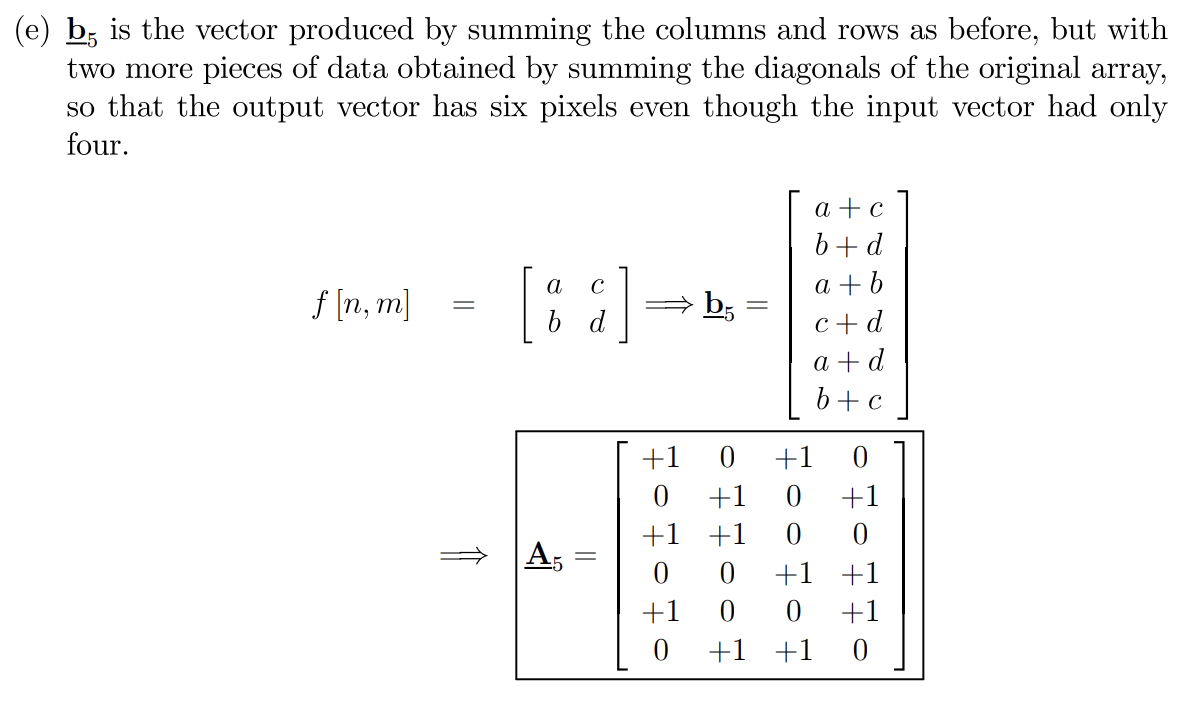
\includegraphics[scale=.65]{Fourier/Week 1/HW/MRI.png}
\caption{Equation from Notes}
\label{fig:Snowman}
\end{figure}



\begin{figure}[h!]
\centering
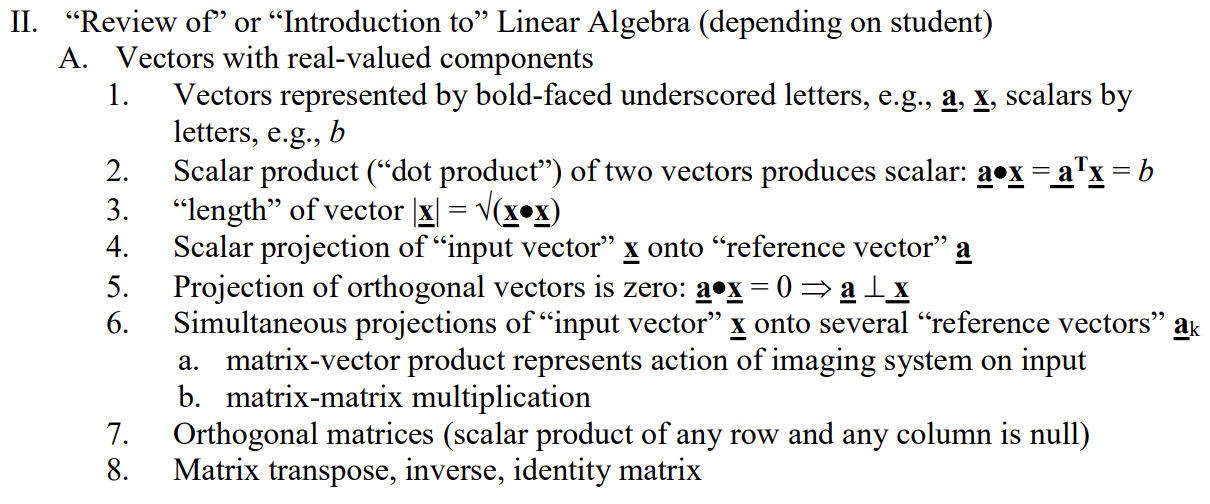
\includegraphics[scale=.65]{Fourier/Week 1/Week1.4.png}
\caption{Easton Syllabus: The basics of Linear Algebra and Matrices}
\label{fig:Snowman}
\end{figure}

\begin{figure}[h!]
\centering
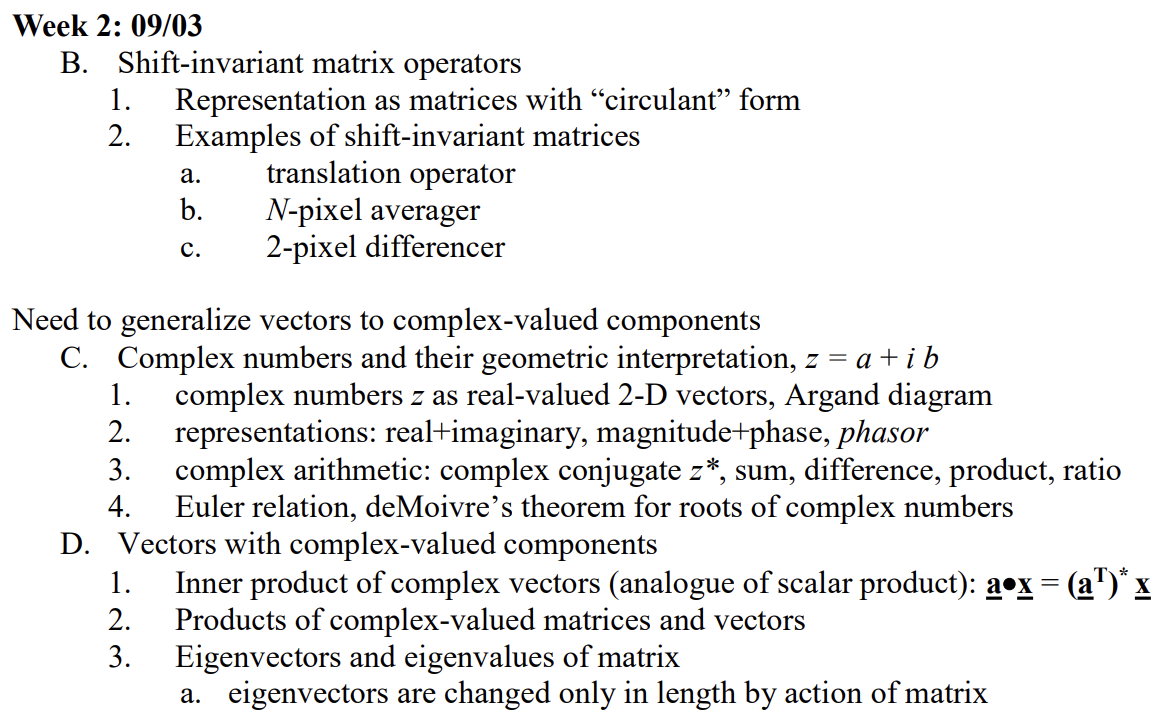
\includegraphics[scale=.65]{Fourier/Week 2/Week2.1.png}
\caption{Easton Syllabus: Argand Diagram and Euler Relation}
\label{fig:Snowman}
\end{figure}

\begin{figure}[h!]
\centering
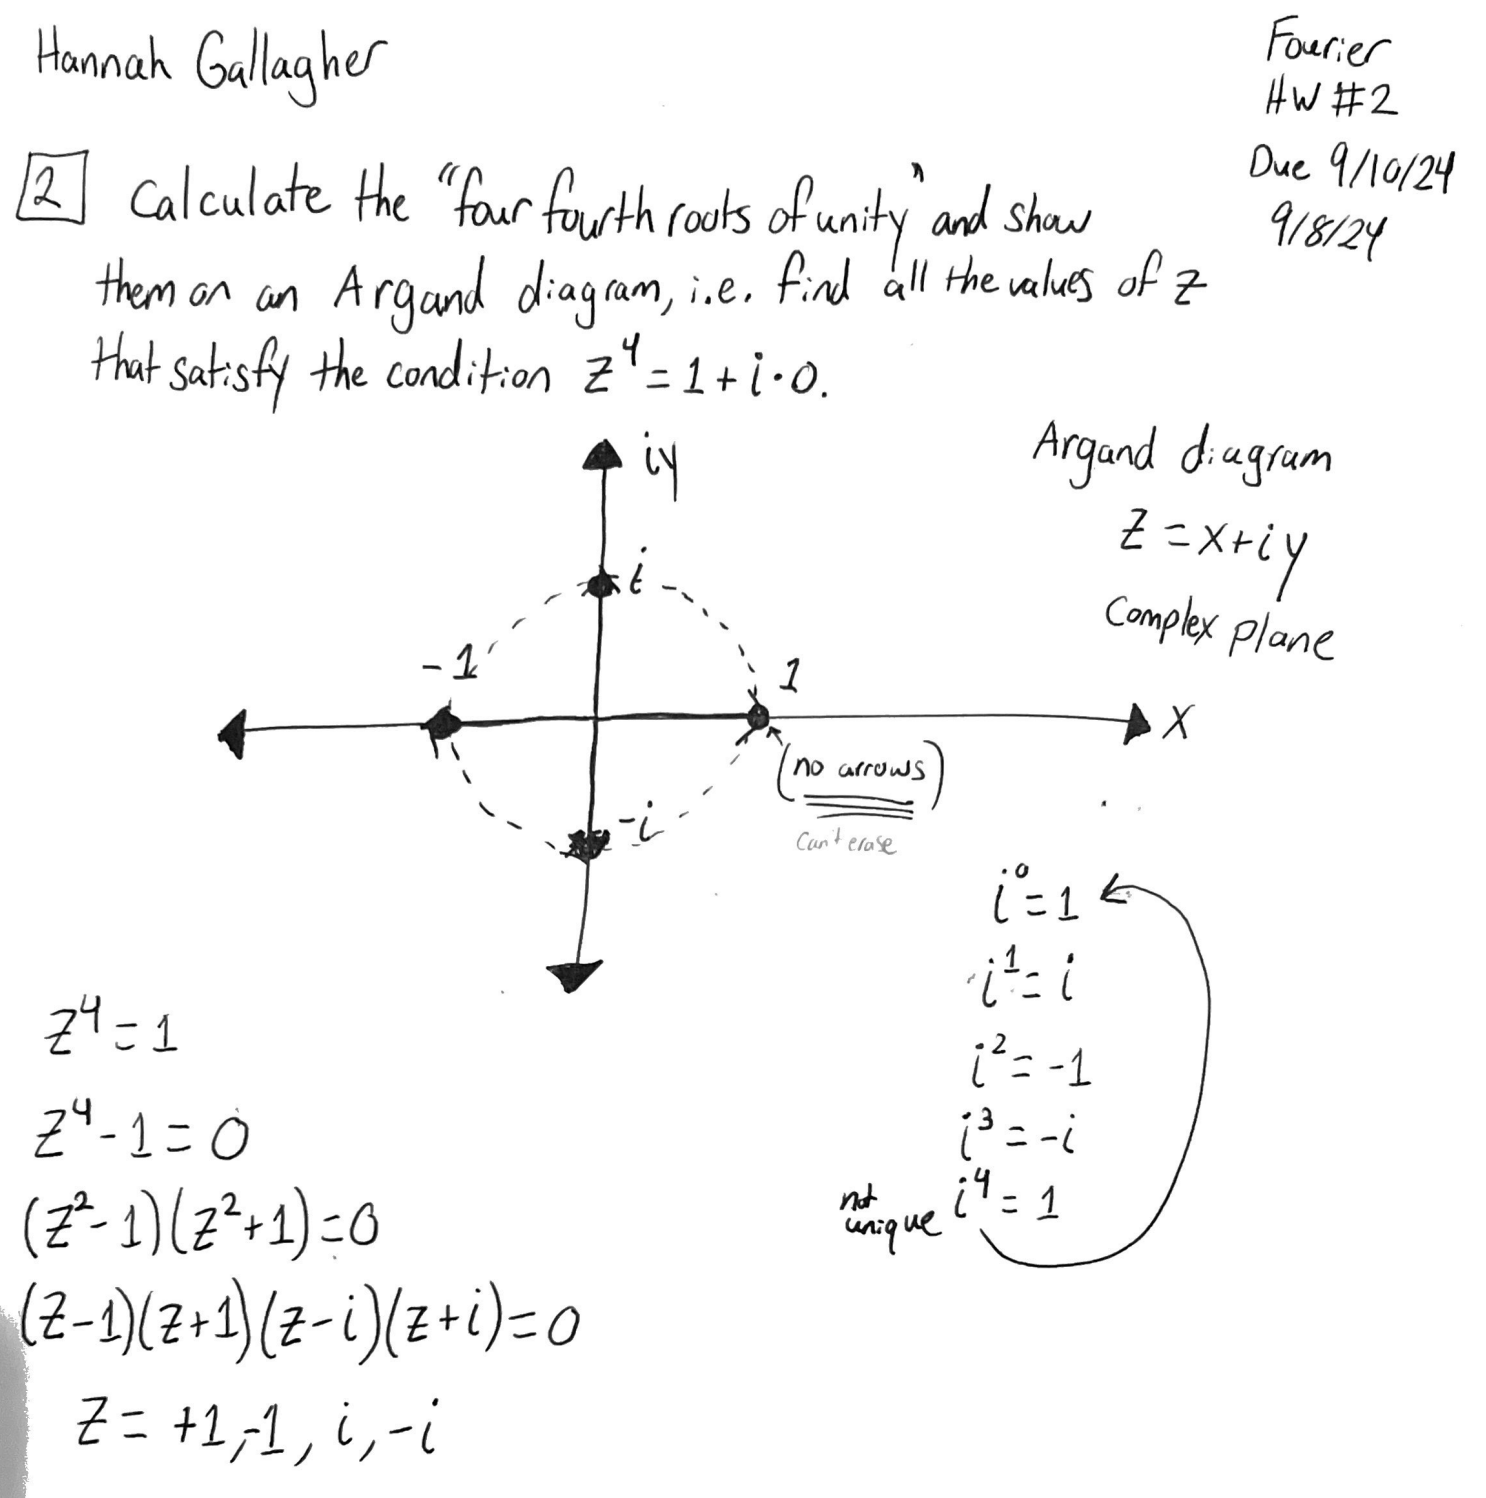
\includegraphics[scale=.4]{Fourier/Week 2/HW/Argand_Roots_of_unity.png}
\caption{Easton Syllabus: Argand Diagram}
\label{fig:Snowman}
\end{figure}


\begin{figure}[h!]
\centering
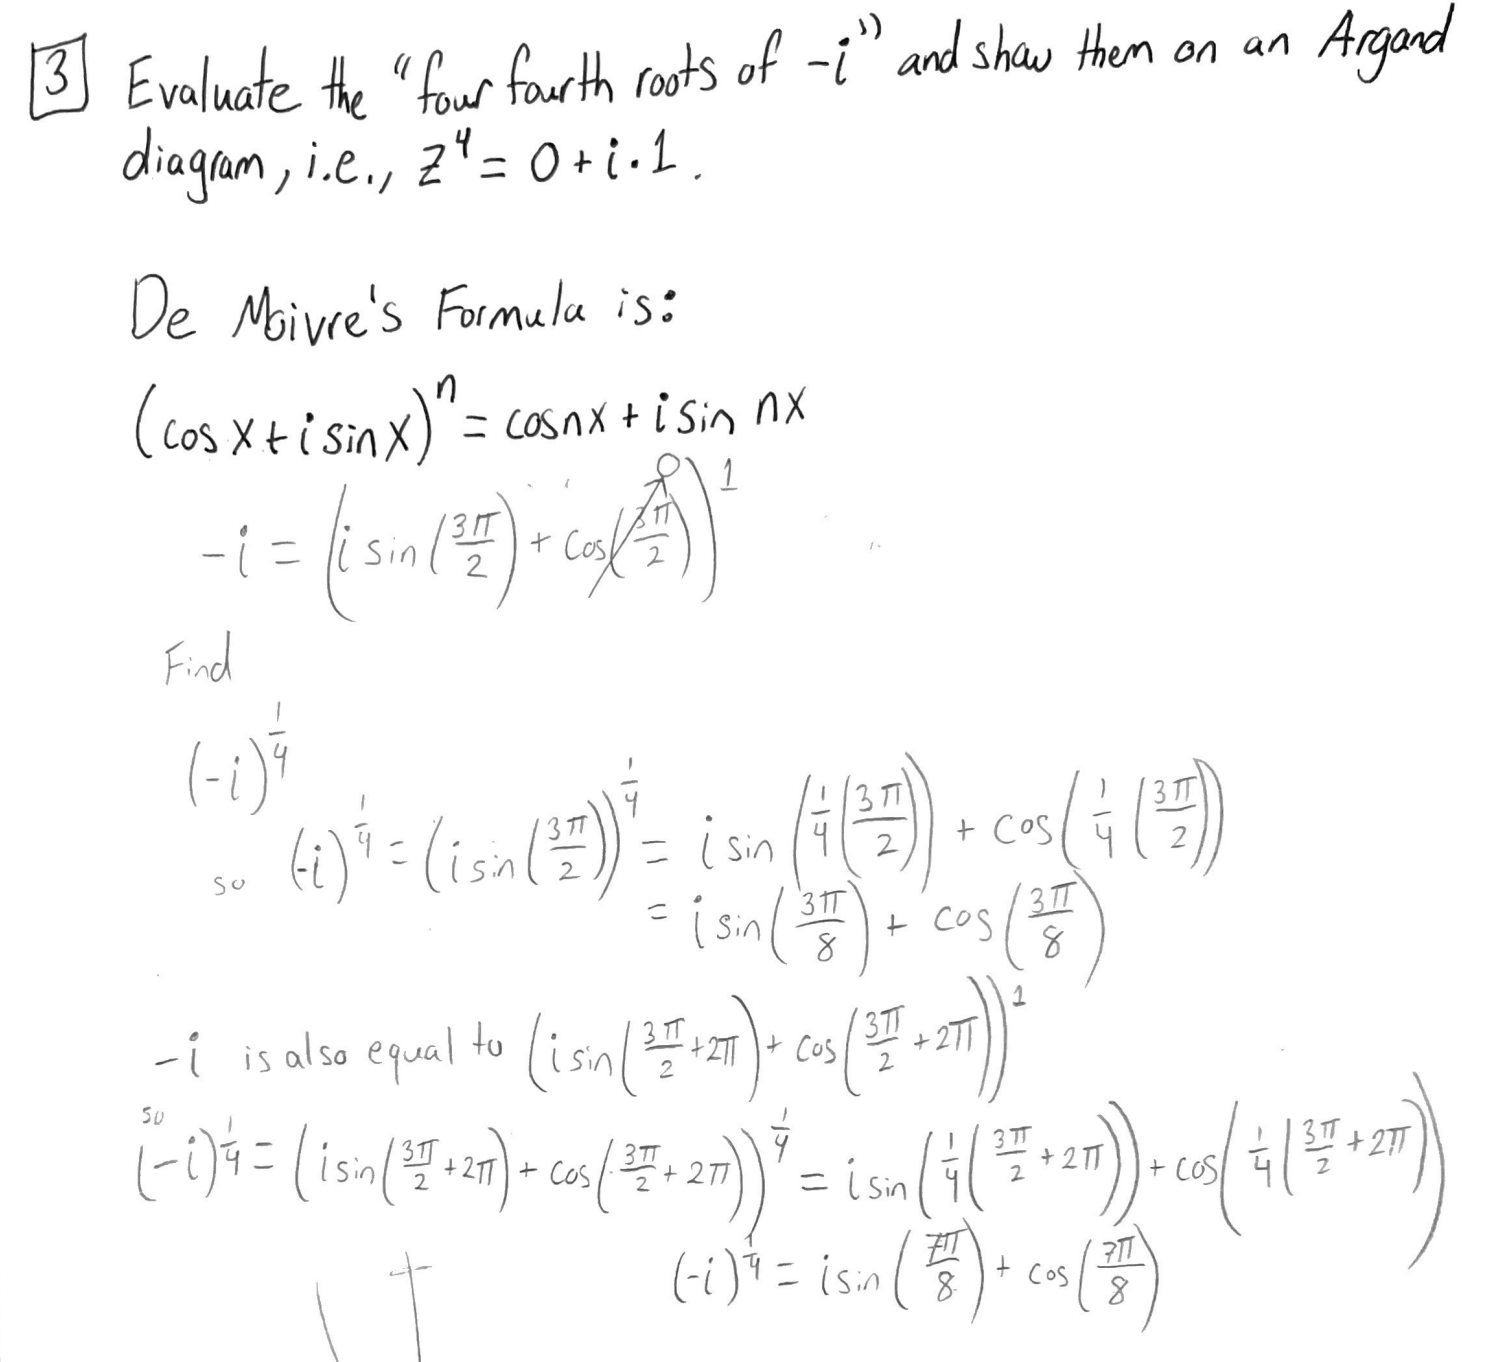
\includegraphics[scale=.65]{Fourier/Week 2/HW/Argand_3.1.png}
\caption{Easton Syllabus: More complicated Argand Diagram:More likely to ask about this. }
\label{fig:Snowman}
\end{figure}

\begin{figure}[h!]
\centering
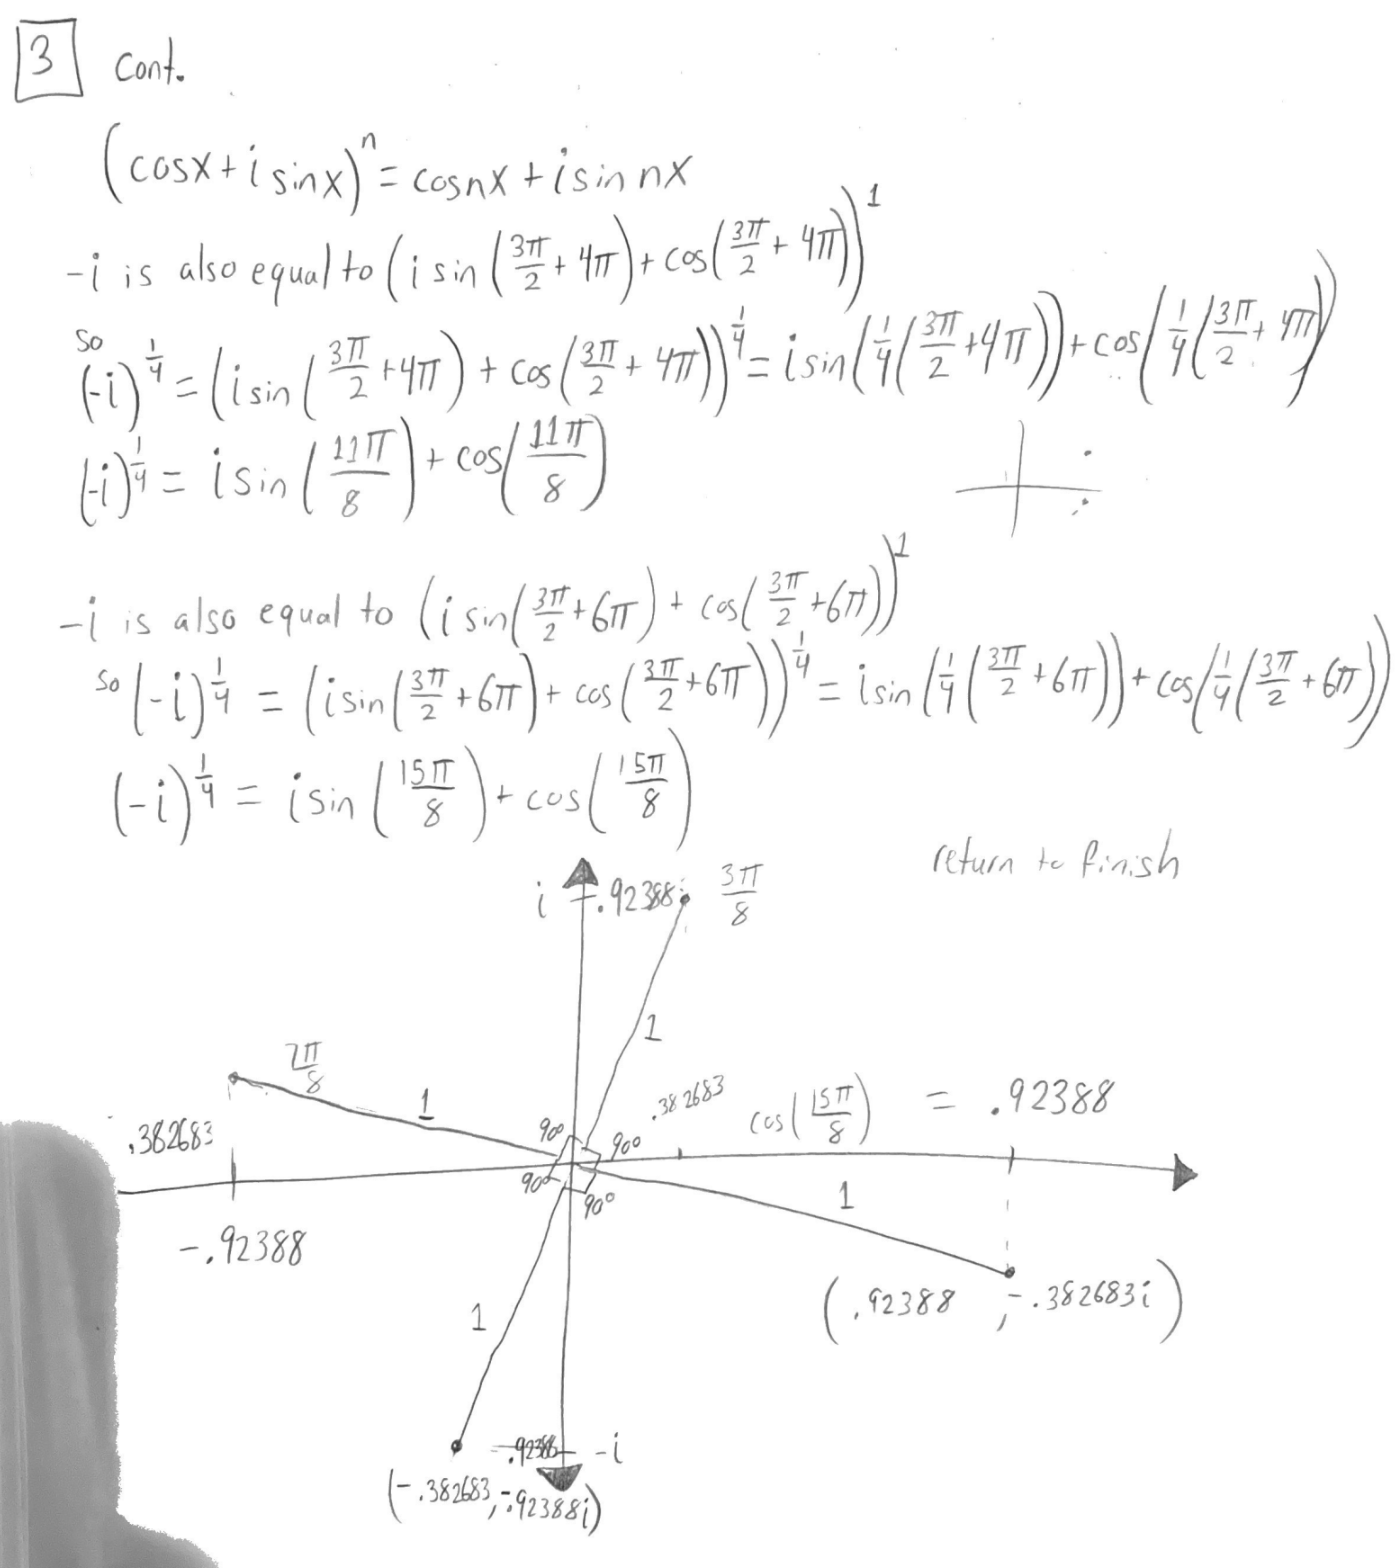
\includegraphics[scale=.65]{Fourier/Week 2/HW/Argand_3.2.png}
\caption{Easton Syllabus: More complicated Argand Diagram:More likely to ask about this. }
\label{fig:Snowman}
\end{figure}


\begin{figure}[h!]
\centering
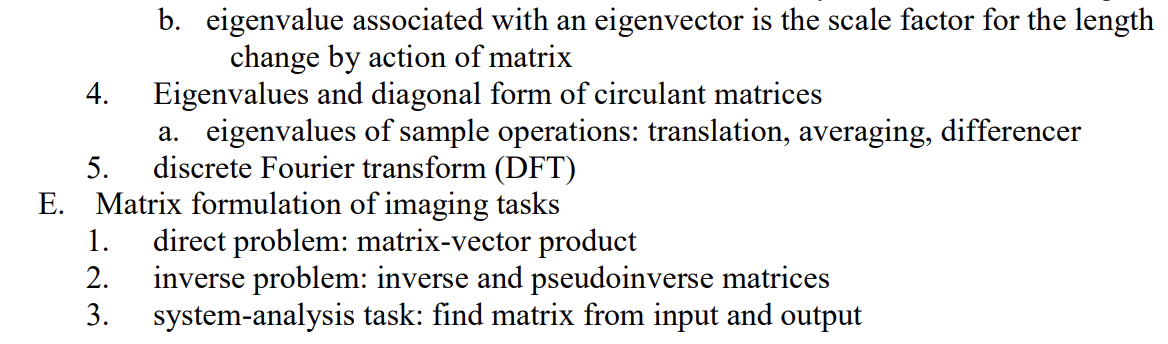
\includegraphics[scale=.65]{Fourier/Week 2/Week2.2.png}
\caption{Easton Syllabus: Pseudoinverse matrices, DFT equation}
\label{fig:Snowman}
\end{figure}
\clearpage
\subsection{Trig Identities}
\begin{equation}
    cos(\theta)= \frac{e^{i \theta}+e^{-i \theta}}{2}
\end{equation}

\begin{equation}
    sin(\theta)= \frac{e^{i \theta}-e^{-i \theta}}{2i}
\end{equation}
Don't forget to remember your adding exponents when their bases are being multiplied by each other!
\begin{equation}
    sin(\theta)= cos(\theta - \frac{\pi}{2}) 
\end{equation}

\begin{figure}[h!]
\centering
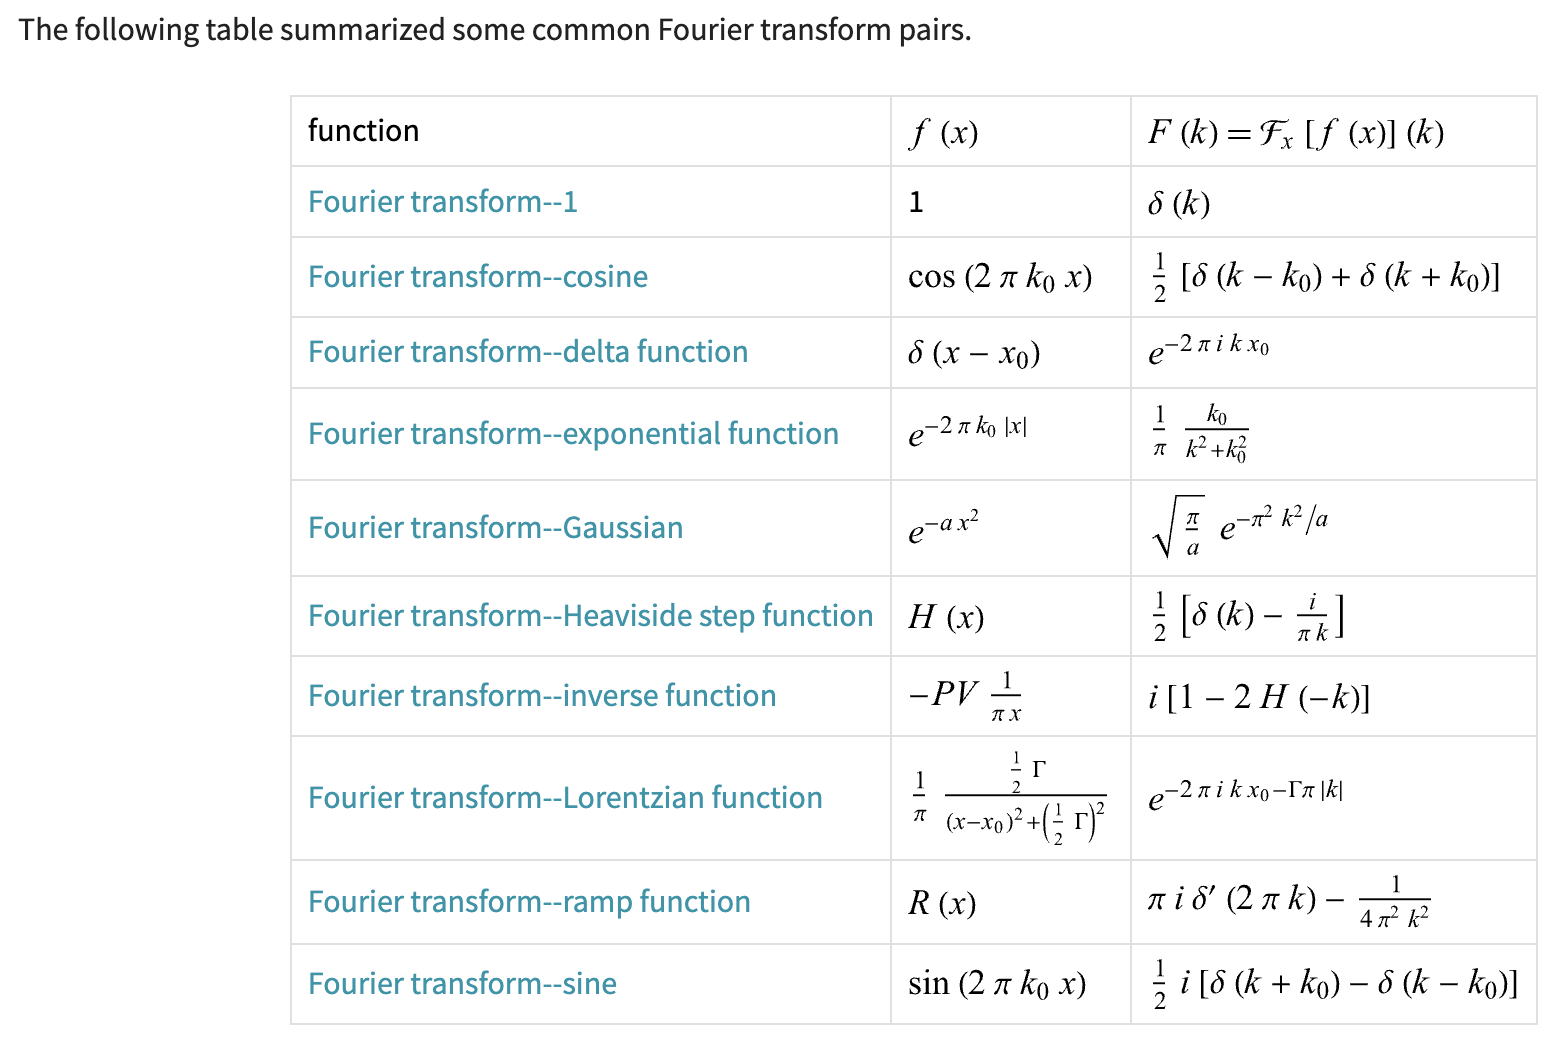
\includegraphics[scale=.65]{Fourier/Week 2/HW/FourierTransformSheet.png}
\caption{Wolfram Quick Reference}
\label{fig:Snowman}
\end{figure}




\begin{figure}[h!]
\centering
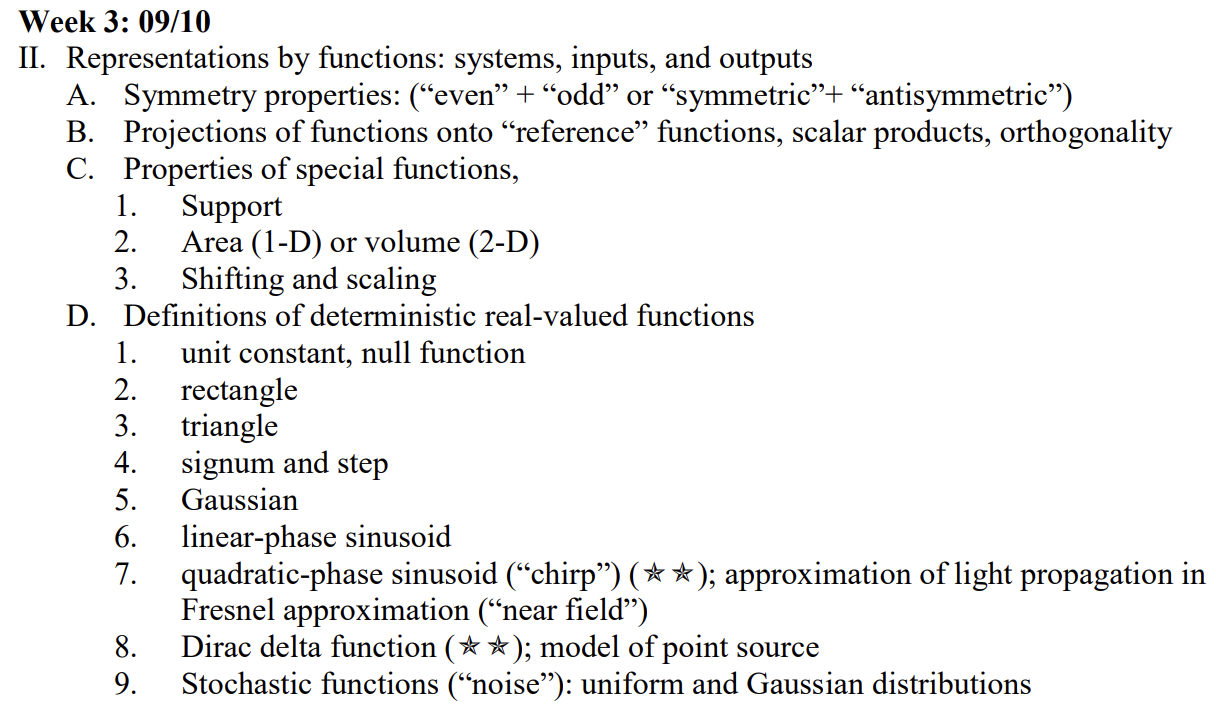
\includegraphics[scale=.65]{Fourier/Week 3/Week3.1.png}
\caption{Easton Syllabus}
\label{fig:Snowman}
\end{figure}

\begin{figure}[h!]
\centering
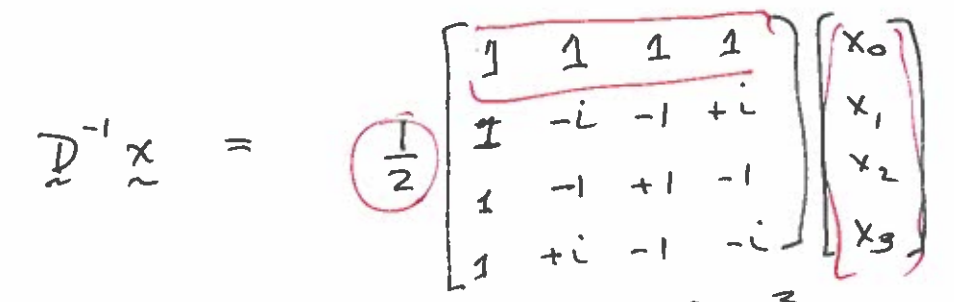
\includegraphics[scale=.65]{Fourier/Week 3/Notes/DMatrix.png}
\caption{The D Inverse Matrix}
\label{fig:Notes3}
\end{figure}

\begin{figure}[h!]
\centering
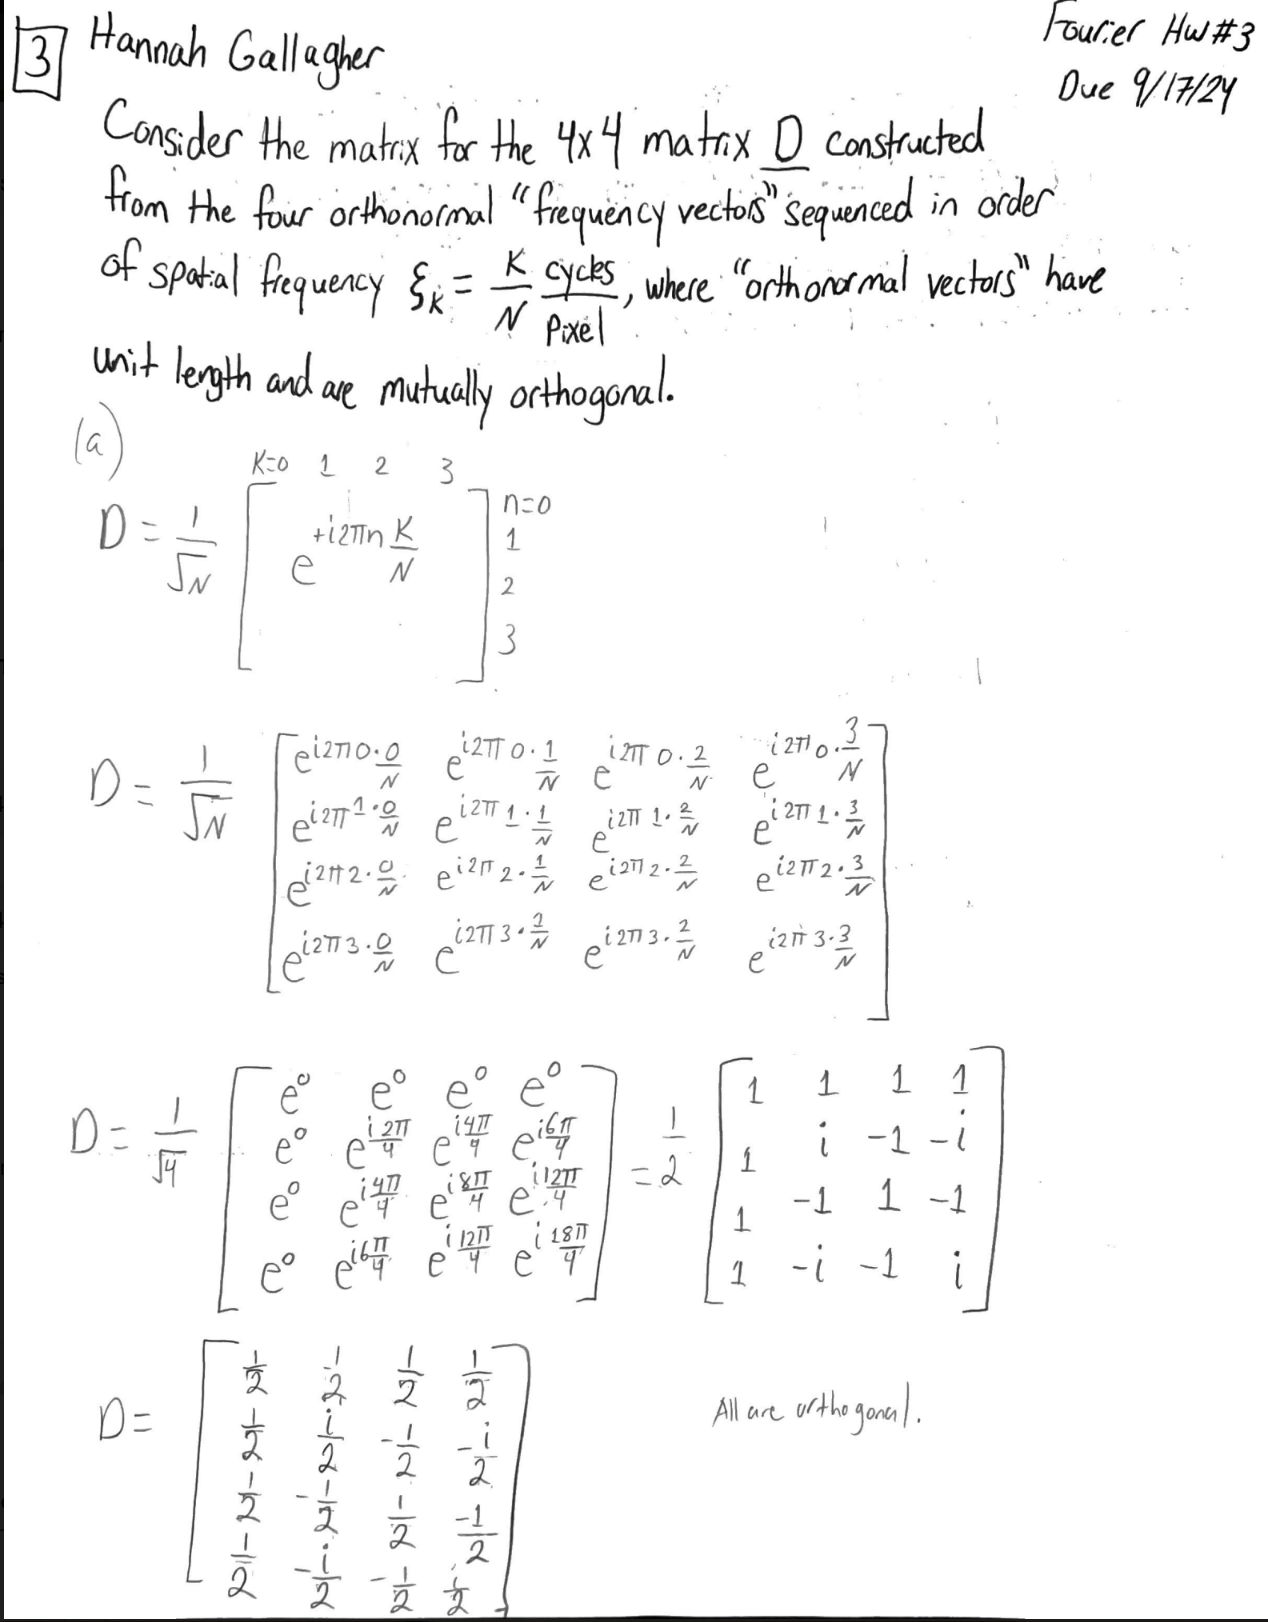
\includegraphics[scale=.65]{Fourier/Week 3/HW/DMatrixHW.png}
\caption{The D Inverse Matrix}
\label{fig:Notes3}
\end{figure}



\begin{figure}[h!]
\centering
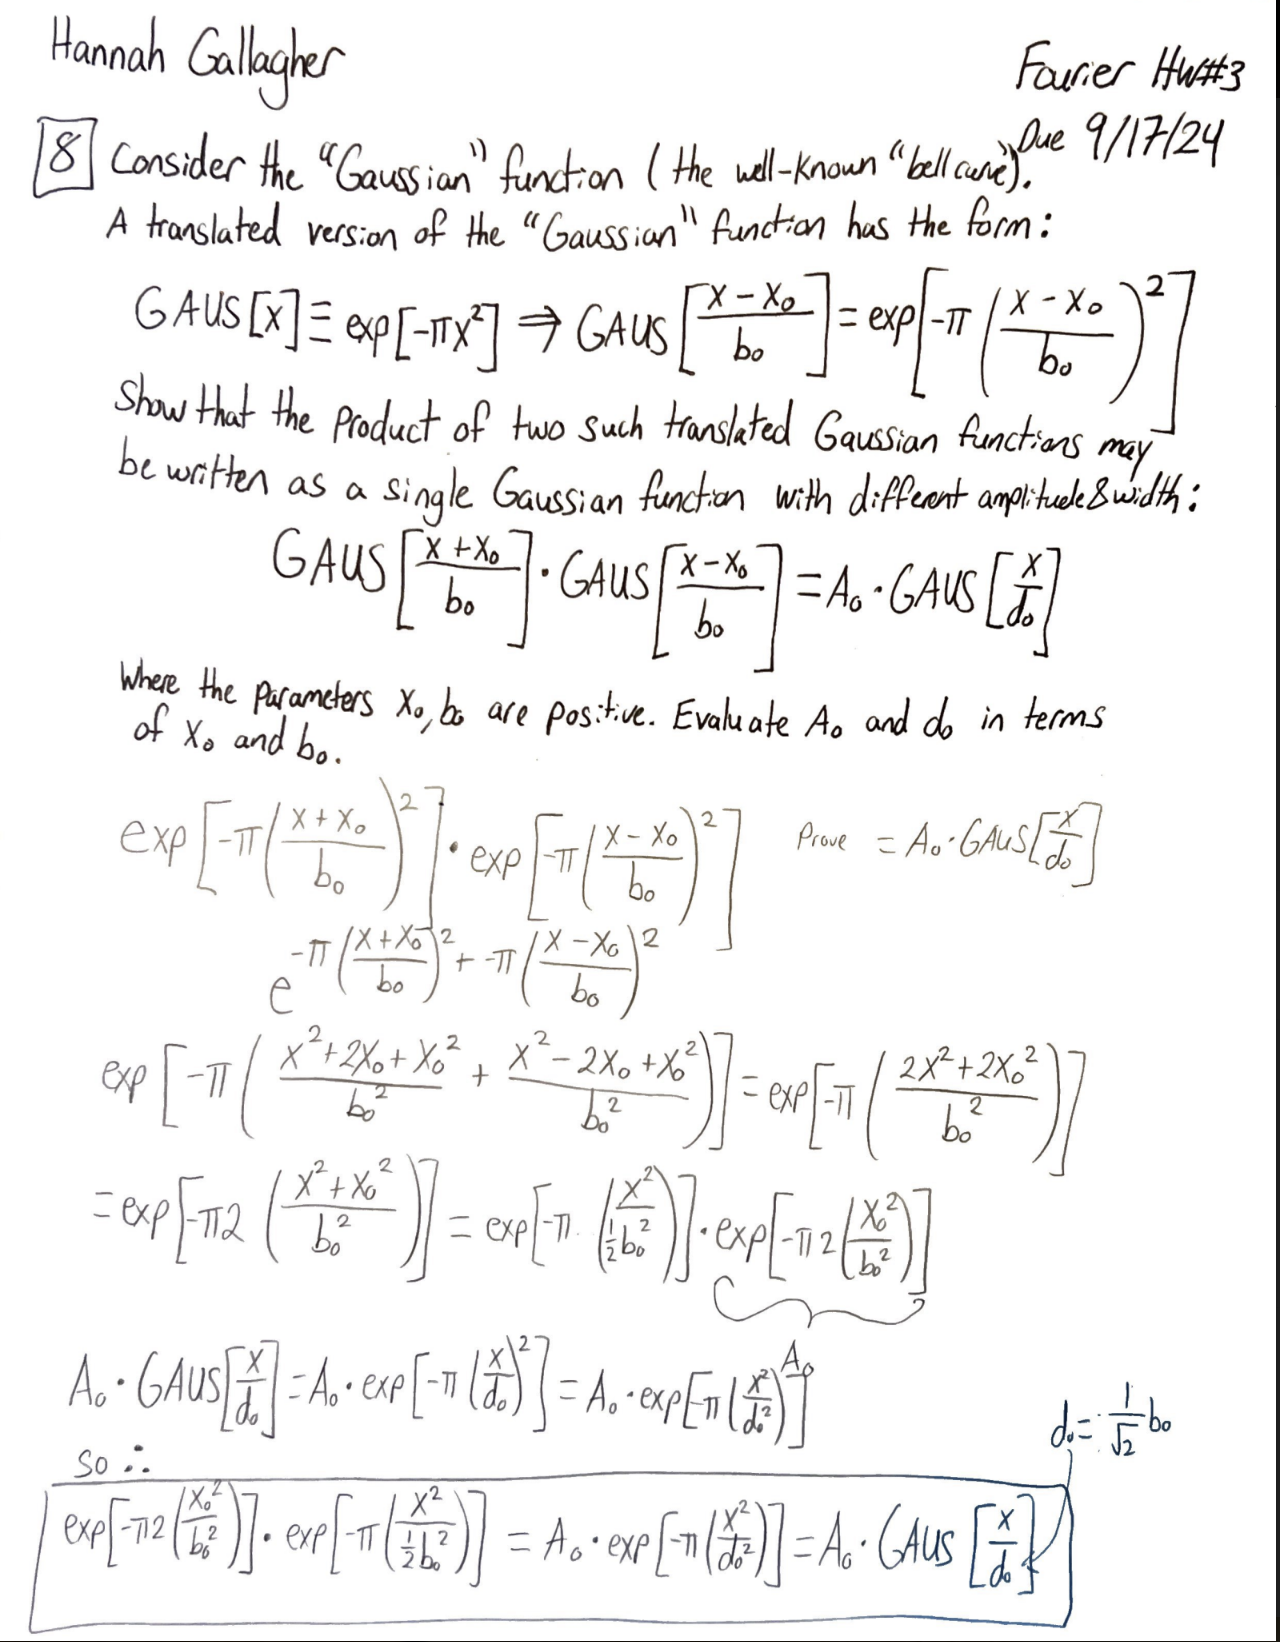
\includegraphics[scale=.65]{Fourier/Week 3/HW/Gaussian.png}
\caption{I'm not exactly why we are deriving this, but you are using the rules of adding exponents that are being multiplied by each other.}
\label{fig:Snowman}
\end{figure}

\begin{figure}[h!]
\centering
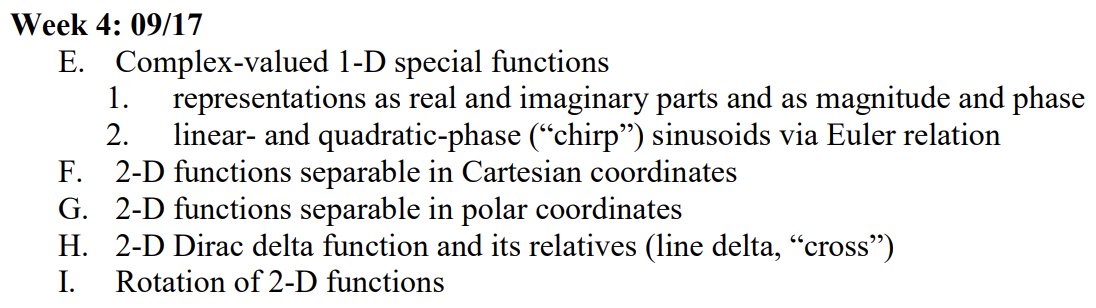
\includegraphics[scale=.65]{Fourier/Week 4/Week4.1.png}
\caption{Easton Syllabus}
\label{fig:Snowman}
\end{figure}

\begin{figure}[h!]
\centering
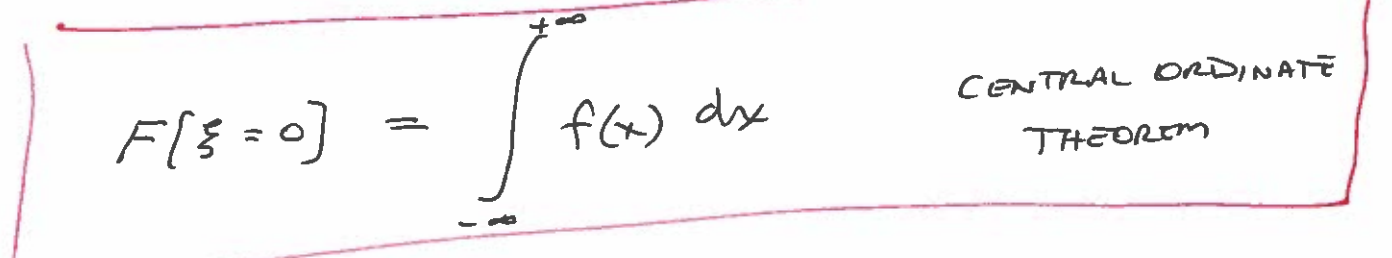
\includegraphics[scale=.65]{Fourier/Week 4/Notes/Ordinate.png}
\caption{Equation from Notes}
\label{fig:Snowman}
\end{figure}

\begin{figure}[h!]
\centering
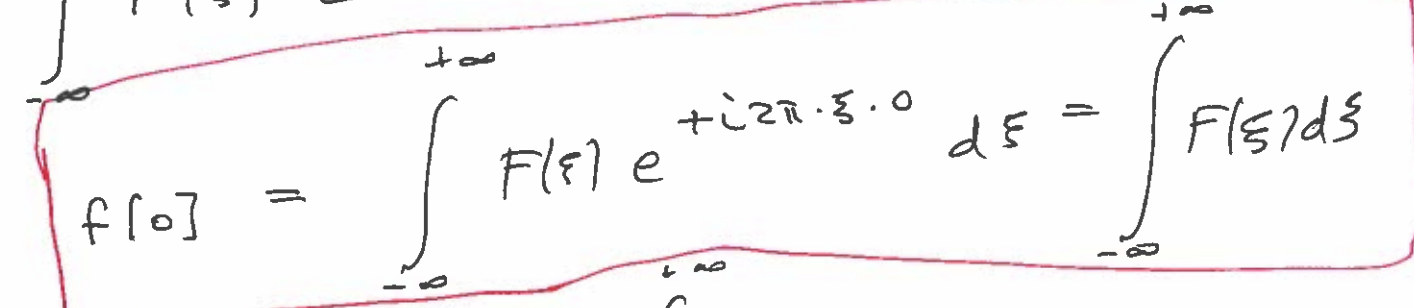
\includegraphics[scale=.65]{Fourier/Week 4/Notes/Formula.png}
\caption{Equation from Notes}
\label{fig:Ordinate}
\end{figure}


\begin{figure}[h!]
\centering
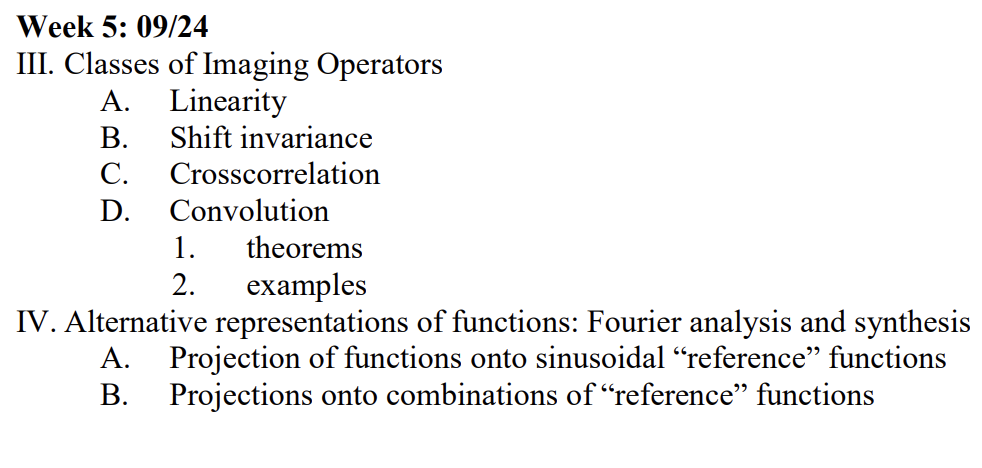
\includegraphics[scale=.65]{Fourier/Week 5/Week5.1.png}
\caption{Easton Syllabus}
\label{fig:Syllabus}
\end{figure}

\begin{figure}[h!]
\centering
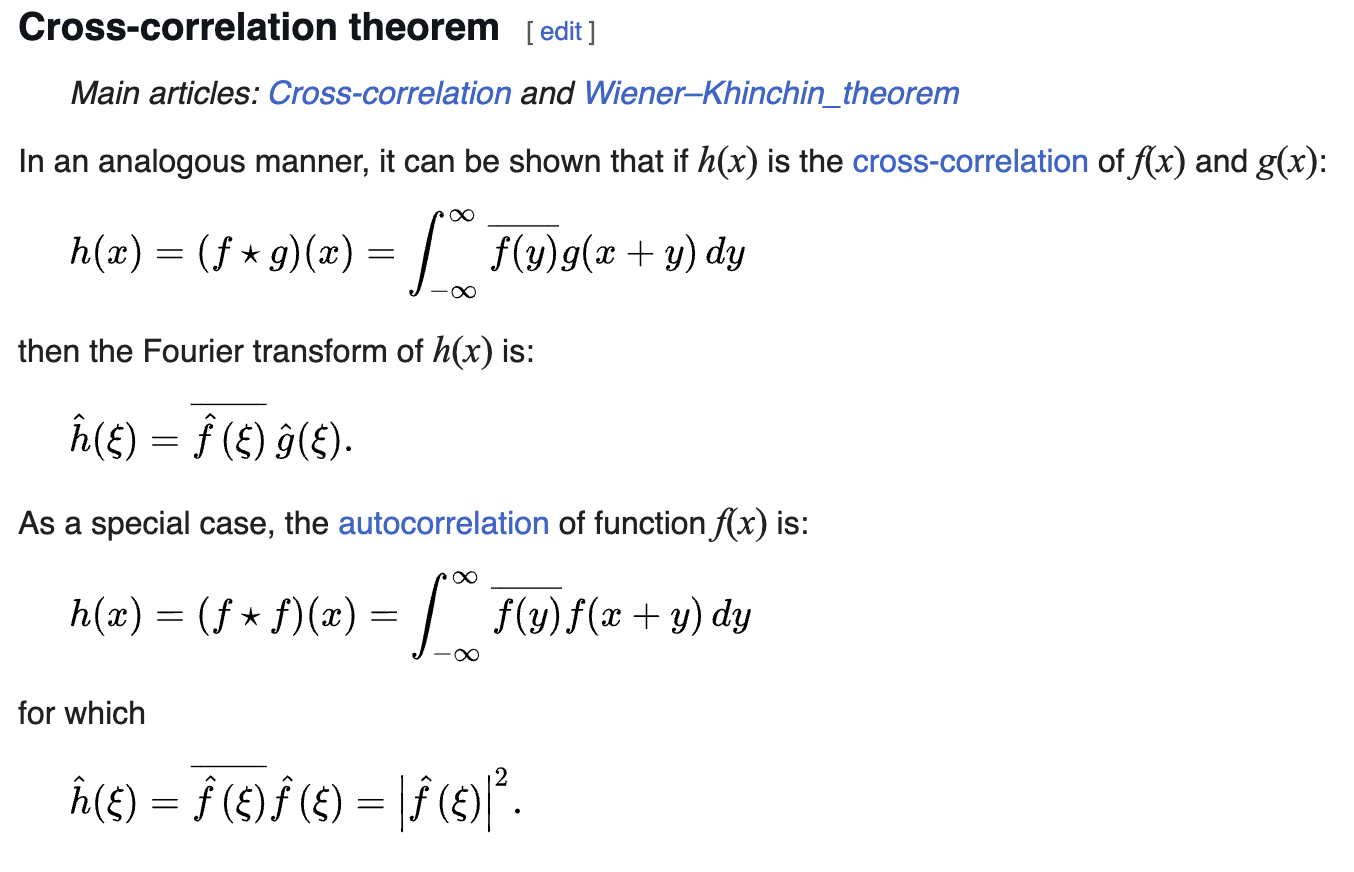
\includegraphics[scale=.65]{Fourier/Week 5/Cross-Correlation_Theorem.png}
\caption{Easton Syllabus}
\label{fig:Syllabus}
\end{figure}


\begin{figure}[h!]
\centering
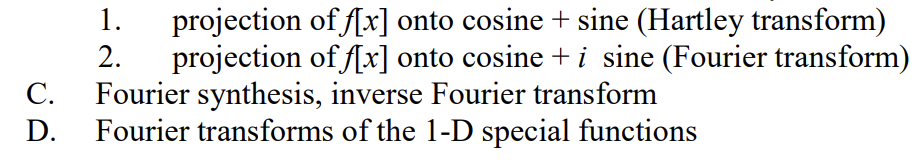
\includegraphics[scale=.65]{Fourier/Week 5/Week5.2.png}
\caption{Easton Syllabus}
\label{fig:Syllabus5}
\end{figure}


\begin{figure}[h!]
\centering
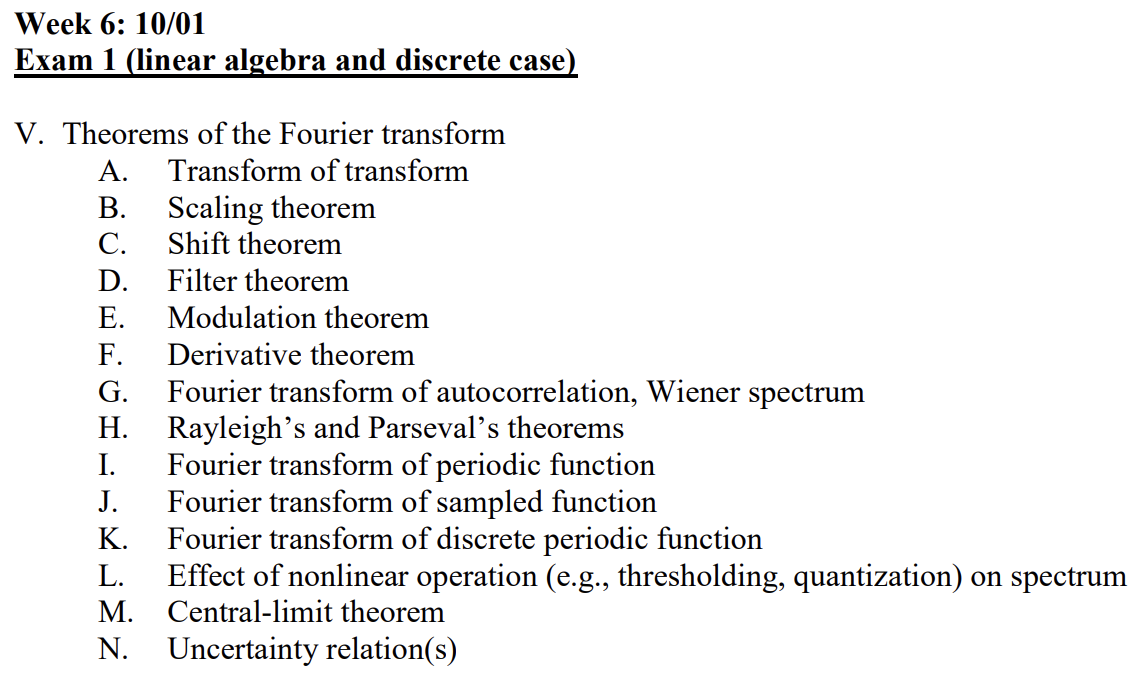
\includegraphics[scale=.65]{Fourier/Week 6/Week6.1.png}
\caption{Easton Syllabus: Wiener Spectrum was emphasized in class.}
\label{fig:Syllabus6}
\end{figure}

\begin{figure}[h!]
\centering
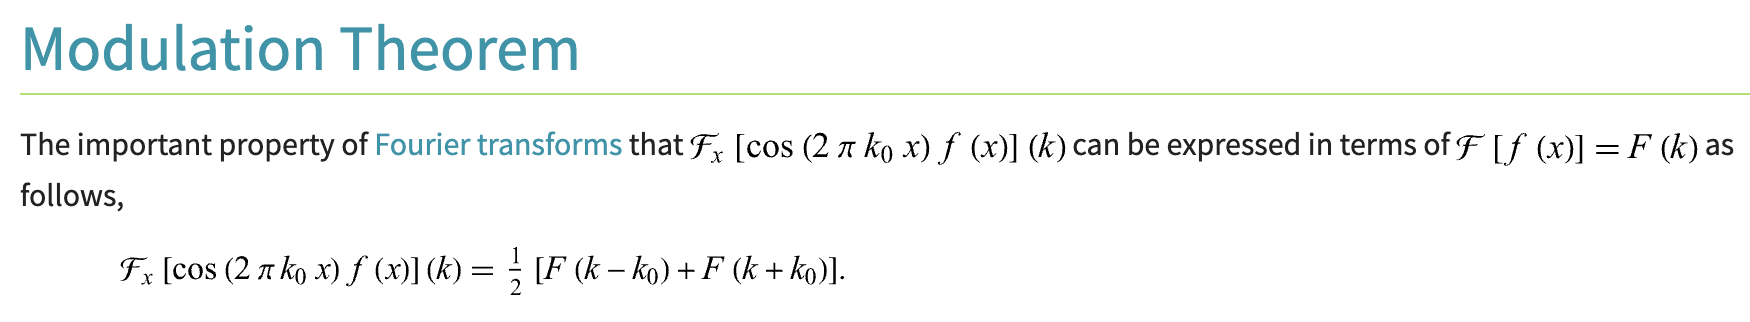
\includegraphics[scale=.55]{Fourier/Week 6/Notes/Modulation.png}
\caption{Modulation Theorem}
\label{fig:Modulation}
\end{figure}

\begin{figure}[h!]
\centering
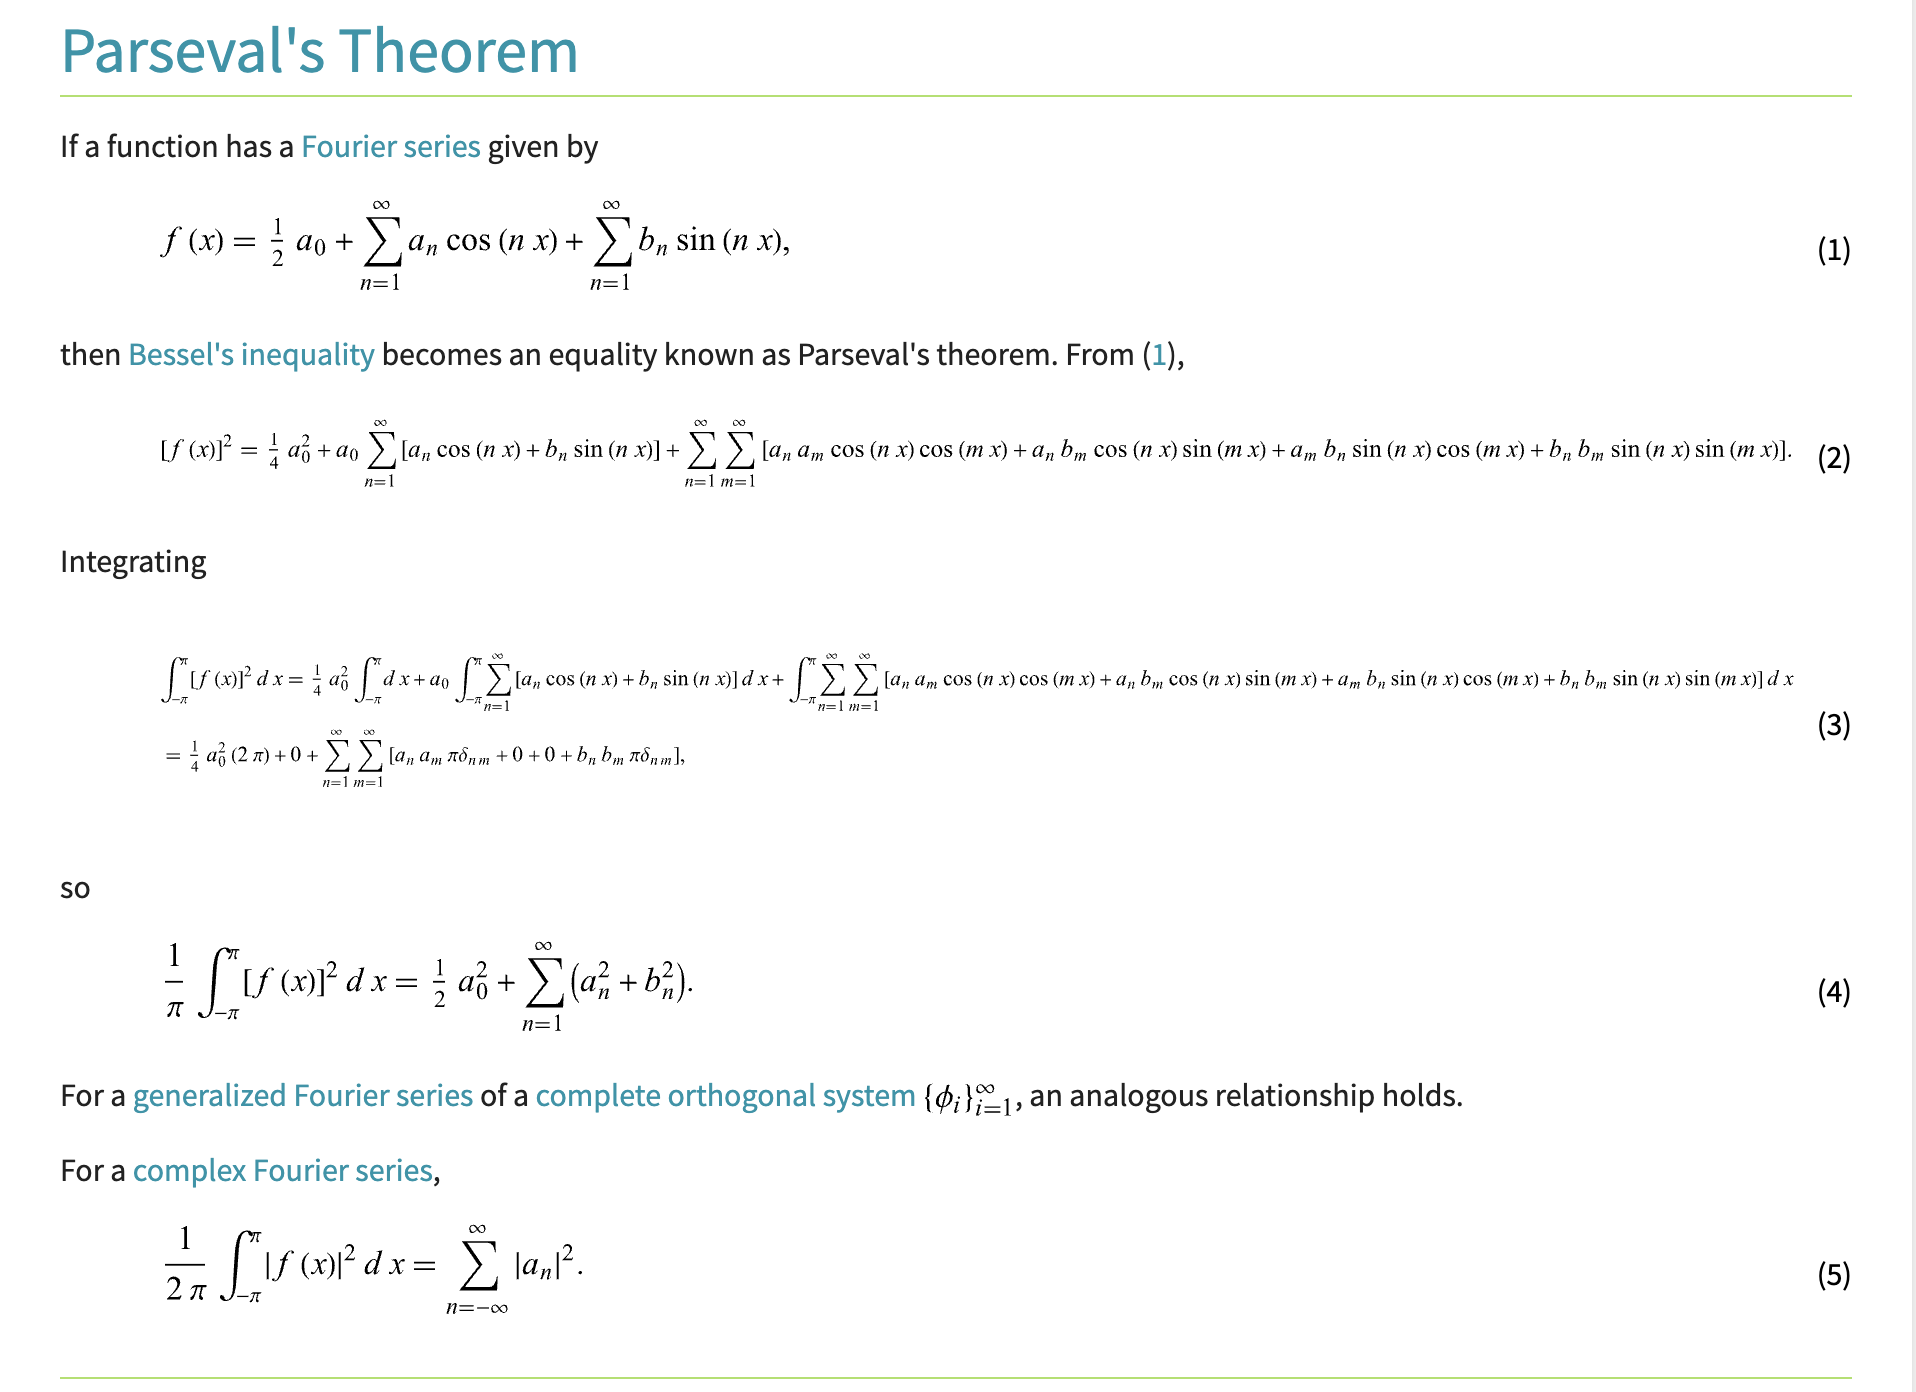
\includegraphics[scale=.55]{Fourier/Week 6/Notes/Parseval.png}
\caption{Parseval Theorem}
\label{fig:Parseval}
\end{figure}




\clearpage
\section{Bibliography}
\begin{thebibliography}{}

\bibitem{Calculus}
Stewart, James. Stewart Calculus. Cengage Learning Emea, 2014.

\bibitem{Fourier}
Easton, Roger Jr. Fourier Methods in Imaging. John Wiley and Sons, Incorporated, 2010.


\end{thebibliography}

\end{document}



